\documentclass[letterpaper, 12pt]{article}

% \usepackage[showframe, margin=1in, top=0.25in, bottom=0.25in, includeheadfoot, headheight=0.5in]{geometry}
\usepackage[margin=1in, top=0.25in, bottom=0.25in, includeheadfoot, headheight=0.5in]{geometry}

\AddToHook{cmd/section/before}{\clearpage}

\usepackage[table]{xcolor}
\colorlet{listingback}{gray!20}
\definecolor{headingcolor}{RGB}{110,34,54}

\usepackage{fancyhdr}
\renewcommand{\sectionmark}[1]{\markboth{#1}{#1}}

% Used to detect whether a section is an appendix to print the right thing in the footer
\usepackage{etoolbox}
\newtoggle{inappendix}
\pretocmd{\appendix}{\clearpage\toggletrue{inappendix}}{}{}

% Save standard definitions for head and foot rules (lines separating header and footer from text)
\let\HeadRule\headrule
\let\FootRule\footrule
% Add color to the standard definitions
\renewcommand{\headrule}{\color{headingcolor}\HeadRule}
\renewcommand{\footrule}{\textcolor{headingcolor}{\FootRule}}

% IMPORTANT: This command should not be called directly. Use \preamble.
% Macro to insert the title page for each lab.
% The argument is the title of the lab.
\newcommand{\inserttitlepage}[1]
{
    \begin{titlepage}
    \centering
    
\includegraphics[scale=0.5]{images/nexus_lab_logo.png}

    \vspace*{\baselineskip}

    \textbf{\Large OpenStack Labs}

    \vspace*{\baselineskip}

    \textbf{\Large #1}
    \vspace*{\fill}
\end{titlepage}
}

% IMPORTANT: This command should not be called directly. Use \preamble.
% Macro to define header and footer for each lab.
% The argument is the title of the lab.
\newcommand{\headfoot}[1]
{
    \fancypagestyle{fancy}
    {
        \fancyhf{}
        \fancyhead[L]{\footnotesize #1}
        \fancyhead[R]{
\includegraphics[height=0.85\headheight]{images/nexus_lab_logo.png}}
        \fancyfoot[L]{%
            \footnotesize%
            \ifnum\value{section}>0%
            \iftoggle{inappendix}{Appendix \thesection: \rightmark}{Section \thesection: \rightmark}%
            \fi}
        \fancyfoot[R]{\footnotesize\thepage}
        \renewcommand{\headrulewidth}{1.5pt}
        \renewcommand{\footrulewidth}{1.5pt}
    }
}

% Macro to insert title page, define header and footer, and insert table of contents and about section for each lab.
% The argument is the title of the lab.
\newcommand{\preamble}[1]
{
    \pagenumbering{roman}
    \inserttitlepage{#1}
    \headfoot{#1}

    % Insert table of contents
    \pagestyle{fancy}
    \tableofcontents
    \clearpage

    \section*{About This Document}
    \label{sec:about_this_document}
    \begin{itemize}
        \item This document was developed by a team at the University of Tennessee at Chattanooga led by Dr. Mengjun Xie
        (\href{mailto:mengjun-xie@utc.edu}{\textbf{mengjun-xie@utc.edu}}).
        \item The development of this document was supported by a National Centers of Academic Excellence in Cybersecurity Grant (\#H98230-20-1-0351), housed at the National Security Agency.
        \item This document is licensed with a Creative Commons Attribution 4.0 International License.
    \end{itemize}
    \clearpage
}

% Macro to insert the Lab Settings page for each lab. Call after the Introduction and Objectives sections.
\newcommand{\labsettings}
{
    \section*{Lab Settings}
    \label{sec:lab_settings}
    \addcontentsline{toc}{section}{\nameref{sec:lab_settings}}
    The information in the table below will be needed in order to complete the lab.
    The task sections below provide details on the use of this information.
    \begin{table*}[htbp]
        \centering
        \begin{tabular}{|c|c|c|c|}
            \hline
            \rowcolor{gray!20} \textbf{Virtual Machine} & \textbf{IP Address} & \textbf{Account} & \textbf{Password} \\
            \hline
            \multirow{2}{*}{\texttt{workstation}} & \multirow[t]{2}{*}{\texttt{ens3: 192.168.1.21}}  & \multirow{2}{*}{\texttt{ubuntu}} & \multirow{2}{*}{\texttt{ubuntu}} \\
                                                  & \multirow[t]{2}{*}{\texttt{ens4: 172.25.250.21}} &                                  &                                  \\
            \hline
            \multirow{2}{*}{\texttt{devstack}}    & \multirow[t]{2}{*}{\texttt{ens3: 192.168.20}}    & \multirow{2}{*}{\texttt{ubuntu}} & \multirow{2}{*}{\texttt{ubuntu}} \\
                                                  & \multirow[t]{2}{*}{\texttt{ens4: 172.25.250.20}} &                                  &                                  \\
            \hline
        \end{tabular}
    \end{table*}
    \clearpage

    % IMPORTANT(lucas): If another frontmatter section ever gets placed after this, this command needs to be moved
    % to the end of that section.
    % I have placed this here and not in each lab purely for convenience and to ensure I don't forget any.
    \pagenumbering{arabic}
}

% Sans-serif font
\renewcommand{\familydefault}{\sfdefault}
\newcommand{\texttildemid}{{\raisebox{0.5ex}{\texttildelow}}}

\usepackage{enumitem}
\renewcommand{\labelenumi}{\textbf{\thesection.\arabic{enumi}.}}

% Try to forbid widows and orphans
\widowpenalty10000
\clubpenalty10000

\usepackage{graphicx}
\usepackage{hyperref}
\hypersetup{colorlinks=true,linkcolor=black,urlcolor={[named] headingcolor}}

\usepackage{sectsty}
\sectionfont{\color{headingcolor}}

% Table of Contents
\usepackage{bookmark}
\usepackage[titles]{tocloft}
\usepackage[title]{appendix}
\renewcommand{\cfttoctitlefont}{\Large\bfseries\color{headingcolor}}
\renewcommand{\cftsecfont}{\normalfont\normalsize}
\renewcommand{\cftsecpagefont}{\normalfont\normalsize}
\renewcommand{\cftdotsep}{0} % Make dots small and close together
\renewcommand{\cftsecleader}{\cftdotfill{\cftdotsep}} % Add dots after section titles
% Make dots go all the way to the page number
\renewcommand{\cftsecfillnum}[1]{{\cftsecleader}\nobreak{\cftsecpagefont #1}\cftsecafterpnum\par}

\usepackage{multirow}
\setlength{\tabcolsep}{16pt}
\renewcommand{\arraystretch}{1.1}

% For nice-looking boxes
\usepackage[most]{tcolorbox}
\usepackage{listings}
\usepackage{lstautogobble}
\lstset{
  frame=none,
  language=Bash,
  showstringspaces=false,
  basicstyle={\linespread{1.1}\footnotesize\ttfamily\selectfont},
  numbers=none,
  breaklines=true,
  breakatwhitespace=true,
  tabsize=3,
  columns=fullflexible,
  keepspaces=true,
  escapeinside={(*@}{@*)},
  literate={~}{{\texttildemid}}{1}
           {\#}{\#}{1},
  autogobble=true
}

\tcolorboxenvironment{lstlisting}
{
    spartan,
    colframe=gray!50,
    boxsep=0mm,
    left=1mm,
    right=1mm,
    top=-1mm,
    bottom=-1mm,
    colback=gray!20
}

% Hacky solution for now, would like to have just one environment and make several tcolorboxes by passing different
% colors as parameters, but that is giving errors
\makeatletter
\tcbset{
  note/.style={%
        enhanced,
        breakable,
        colback=blue!10!white,
        colframe=blue!80!white,
        attach boxed title to top left={yshift*=-\tcboxedtitleheight},
        title={#1},
        boxed title size=title,
        boxed title style={%
            sharp corners,
            rounded corners=northwest,
            colback=tcbcolframe,
            boxrule=0pt,
        },
        underlay boxed title={%
            \path[fill=tcbcolframe] (title.south west)--(title.south east)
                to[out=0, in=180] ([xshift=5mm]title.east)--
                (title.center-|frame.east)
                [rounded corners=\kvtcb@arc] |-
                (frame.north) -| cycle;
        },
    }
}
\makeatother

\makeatletter
\tcbset{
    stop/.style={%
        enhanced,
        breakable,
        colback=white,
        colback=red!10!white,
        colframe=red!80!white,
        attach boxed title to top left={yshift*=-\tcboxedtitleheight},
        title={#1},
        boxed title size=title,
        boxed title style={%
            sharp corners,
            rounded corners=northwest,
            colback=tcbcolframe,
            boxrule=0pt,
        },
        underlay boxed title={%
            \path[fill=tcbcolframe] (title.south west)--(title.south east)
                to[out=0, in=180] ([xshift=5mm]title.east)--
                (title.center-|frame.east)
                [rounded corners=\kvtcb@arc] |-
                (frame.north) -| cycle;
        },
    }
}
\makeatother

\makeatletter
\tcbset{
    tip/.style={%
        enhanced,
        breakable,
        colback=white,
        colback=green!10,
        colframe=green!70!black,
        attach boxed title to top left={yshift*=-\tcboxedtitleheight},
        fonttitle=\bfseries,
        title={#1},
        boxed title size=title,
        boxed title style={%
            sharp corners,
            rounded corners=northwest,
            colback=tcbcolframe,
            boxrule=0pt,
        },
        underlay boxed title={%
            \path[fill=tcbcolframe] (title.south west)--(title.south east)
                to[out=0, in=180] ([xshift=5mm]title.east)--
                (title.center-|frame.east)
                [rounded corners=\kvtcb@arc] |-
                (frame.north) -| cycle;
        },
    }
}
\makeatother

% The commands below define environments for colored boxes. They are used like
% \begin{notebox}
% ...
% \end{notebox}
\newtcolorbox{notebox}{note={Note}}
\newtcolorbox{stopbox}{stop={Stop}}
\newtcolorbox{tipbox}{tip={Tip}}


\begin{document}
\begin{titlepage}
    \centering
    
\includegraphics[scale=0.5]{images/nexus_lab_logo.png}

    \vspace*{\baselineskip}

    \textbf{\Large OpenStack Labs}

    \vspace*{\baselineskip}

    \textbf{\Large Lab 6: Deploying an FTP Server}
    \vspace*{\fill}
\end{titlepage}

\fancypagestyle{fancy}
{
    \fancyhf{}
    \fancyhead[L]{\footnotesize Lab 6: Deploying an FTP Server}
    \fancyhead[R]{
\includegraphics[height=0.85\headheight]{images/nexus_lab_logo.png}}
    \fancyfoot[R]{\footnotesize\thepage}
    \renewcommand{\headrulewidth}{0pt}
}

\pagestyle{fancy}
\tableofcontents
\clearpage

\section*{Introduction}
\label{sec:introduction}
\addcontentsline{toc}{section}{\nameref{sec:introduction}}
In this lab, you will practice and demonstrate the knowledge and skills you acquired throughout the course by deploying
an FTP server through OpenStack.

\section*{Objectives}
\label{sec:objectives}
\addcontentsline{toc}{section}{\nameref{sec:objectives}}
\begin{itemize}[itemsep=0pt]
    \item Launch an instance in your OpenStack environment and customize the instance to run an FTP server.
    \item Access the FTP server from the workstation to confirm the configuration.
\end{itemize}
\clearpage

\section*{Lab Settings}
\label{sec:lab_settings}
\addcontentsline{toc}{section}{\nameref{sec:lab_settings}}
The information in the table below will be needed in order to complete the lab. The task sections below provide details
on the use of this information.
\begin{table*}[htbp]
\centering
\begin{tabular}{|c|c|c|c|}
    \hline
    \rowcolor{gray!20} \textbf{Virtual Machine} & \textbf{IP Address} & \textbf{Account} & \textbf{Password} \\
    \hline
    \multirow{2}{*}{\texttt{workstation}} & \multirow[t]{2}{*}{\texttt{ens3: 192.168.1.21}}  & \multirow{2}{*}{\texttt{ubuntu}} & \multirow{2}{*}{\texttt{ubuntu}} \\
                                          & \multirow[t]{2}{*}{\texttt{ens4: 172.25.250.21}} &                                  &                                  \\
    \hline
    \multirow{2}{*}{\texttt{devstack}}    & \multirow[t]{2}{*}{\texttt{ens3: 192.168.1.20}}  & \multirow{2}{*}{\texttt{ubuntu}} & \multirow{2}{*}{\texttt{ubuntu}} \\
                                          & \multirow[t]{2}{*}{\texttt{ens4: 172.25.250.20}} &                                  &                                  \\
    \hline
\end{tabular}
\end{table*}
\clearpage

\section{Launch an FTP Server Instance}
\label{sec:launch_an_ftp_server_instance}
In this task, you will deploy an FTP server in your environment. The architecture will be comprised of an external
network and an internal network, a new privileged user and a non-privileged user, and a set of new security rules to
allow FTP access to the instance. A floating IP will be associated with the instance to permit external connectivity.

\begin{enumerate}
    \item Log into the \textbf{workstation} machine as \textbf{ubuntu} with the password \textbf{ubuntu}.

    \item Open a terminal window and source the \textbf{\texttildemid/keystonerc-admin} keystone credentials file.
\begin{lstlisting}
ubuntu@workstation:~$ source ~/kesytonerc-admin
\end{lstlisting}

    \begin{center}
        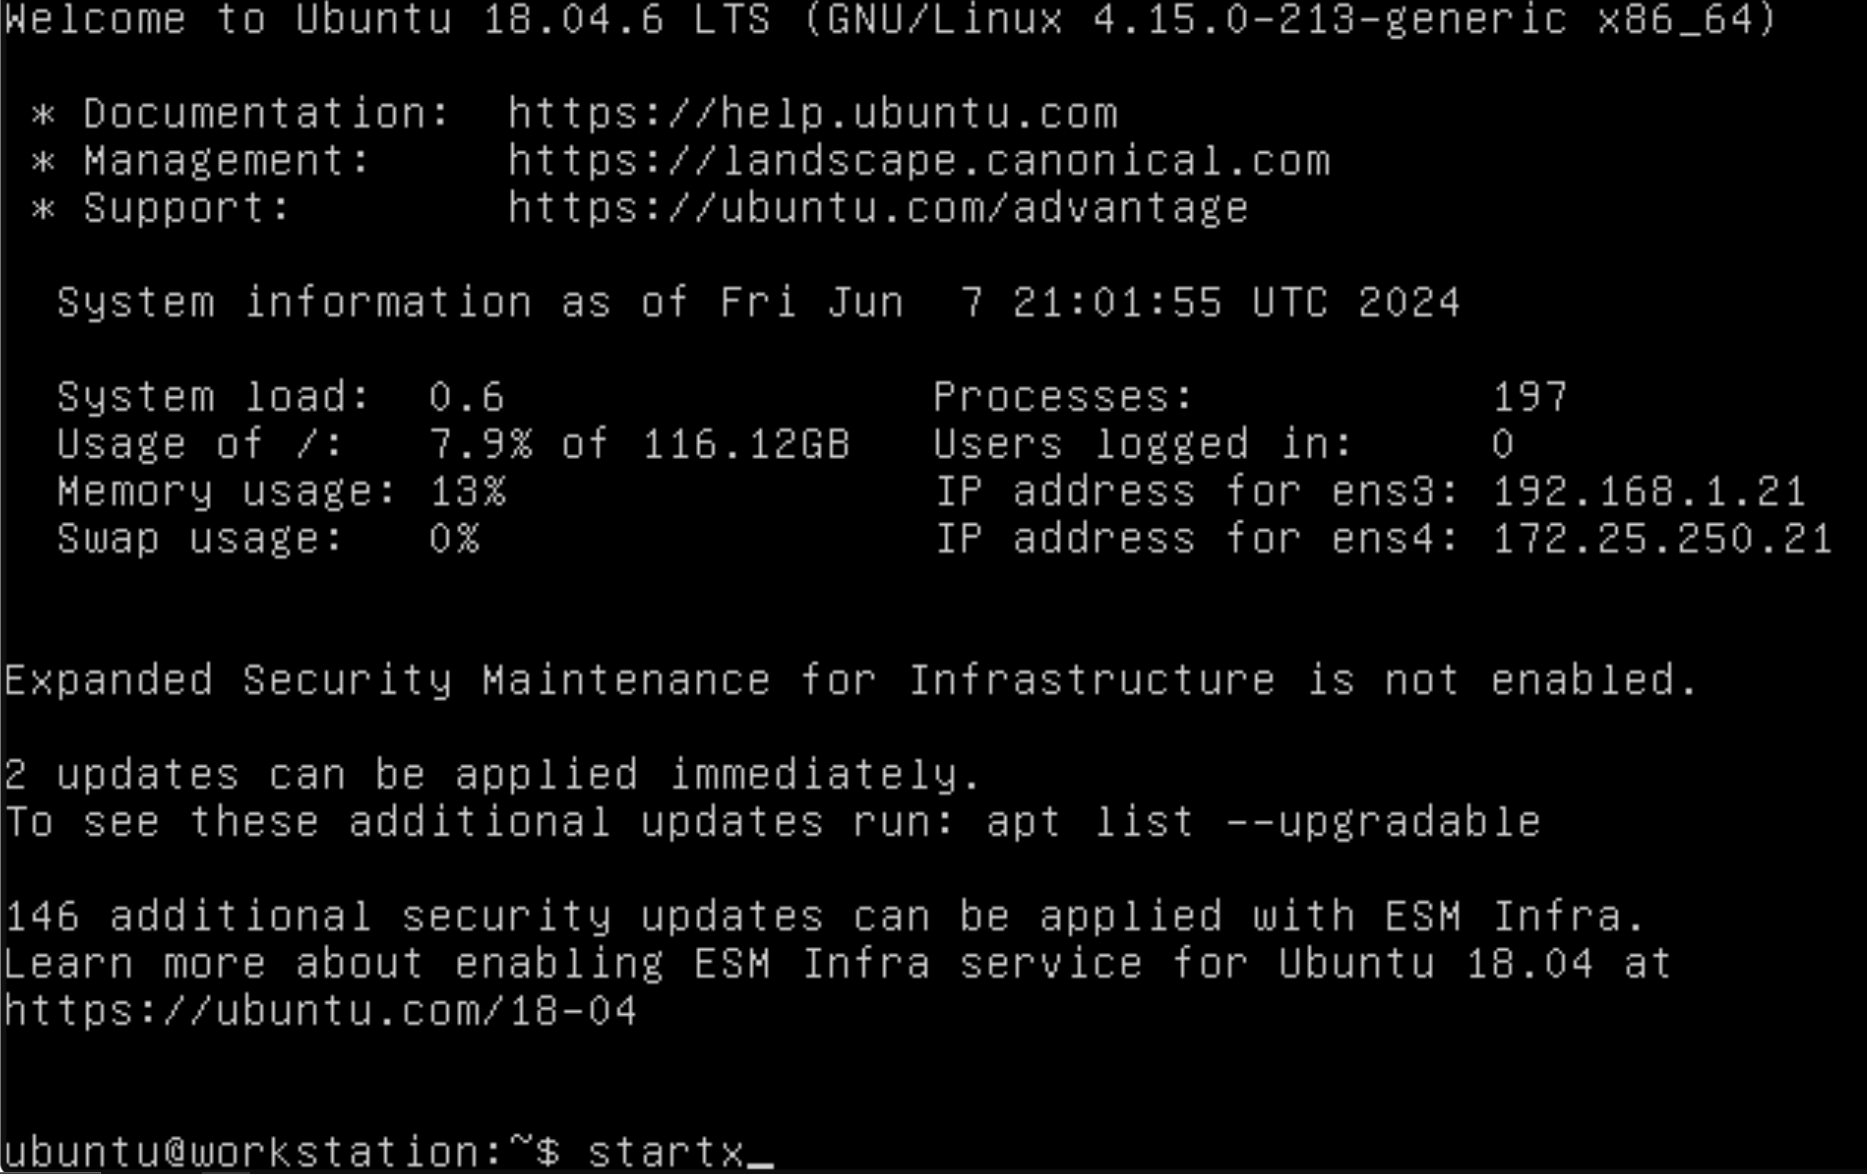
\includegraphics[width=\linewidth]{images/part1/step2.png}
    \end{center}

    \item Delete the \textbf{ubuntu} image.
\begin{lstlisting}
ubuntu@workstation:~$ openstack image delete ubuntu
\end{lstlisting}

\begin{center}
    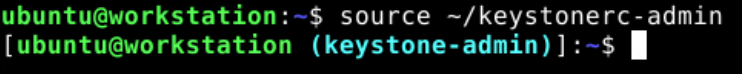
\includegraphics[width=\linewidth]{images/part1/step3.png}
\end{center}

    \item Create the \textbf{prod} project.
\begin{lstlisting}
ubuntu@workstation:~$ openstack project create prod \
> --domain default
\end{lstlisting}

    \begin{center}
        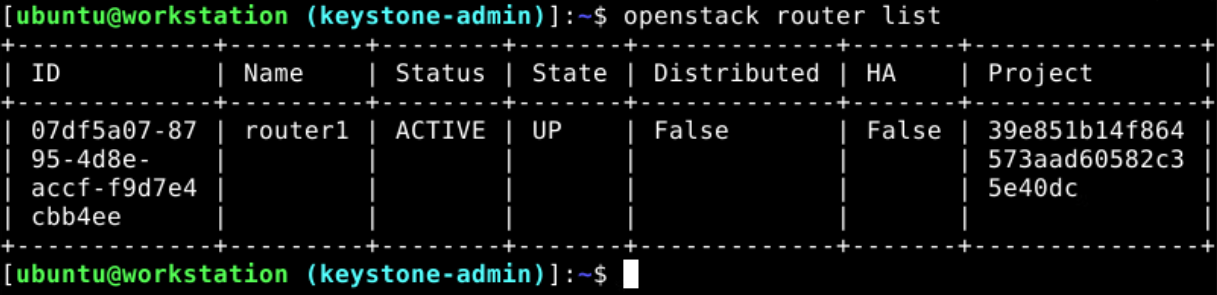
\includegraphics[width=\linewidth]{images/part1/step4.png}
    \end{center}

\begin{tipbox}{}
    When typing the command, make sure there is a space between \texttt{prod} and the \texttt{\textbackslash}
    character, and press \textbf{Enter} to get the \texttt{>} and continue typing the rest of the command.
\end{tipbox}

    \item Create a user named \textbf{superuser} with the password \textbf{secret} to the \textbf{prod} project.
\begin{lstlisting}
ubuntu@workstation:~$ openstack user create \
> --project prod \
> --password secret \
> --email ubuntu@workstation.lab.example.com \
> superuser
\end{lstlisting}

\begin{center}
    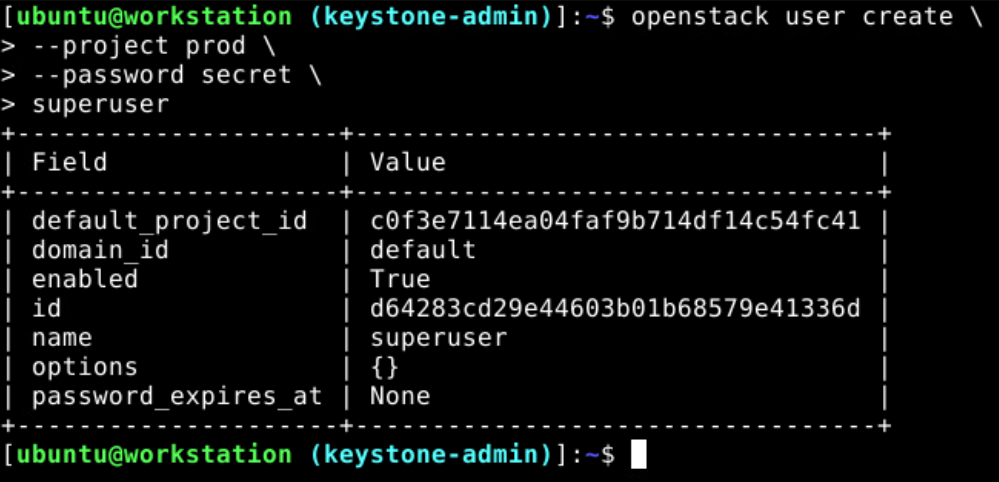
\includegraphics[width=\linewidth]{images/part1/step5.png}
\end{center}

    \item Assign the \textbf{admin} role to the user \textbf{superuser}.
\begin{lstlisting}
ubuntu@workstation:~$ openstack role add \
> --project prod \
> --user superuser \
> admin
\end{lstlisting}

    \begin{center}
        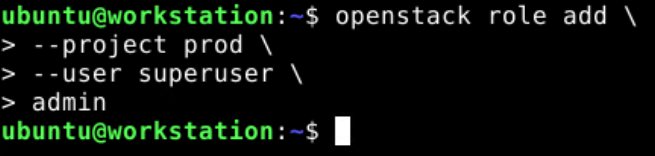
\includegraphics[width=\linewidth]{images/part1/step6.png}
    \end{center}

    \item Copy the keystone credentials file \textbf{\texttildemid/keystonerc-admin} to
    \textbf{\texttildemid/keystonerc-superuser}.
\begin{lstlisting}
ubuntu@workstation~$ cp ~/keystonerc-admin ~/keystonerc-superuser
\end{lstlisting}

    \begin{center}
        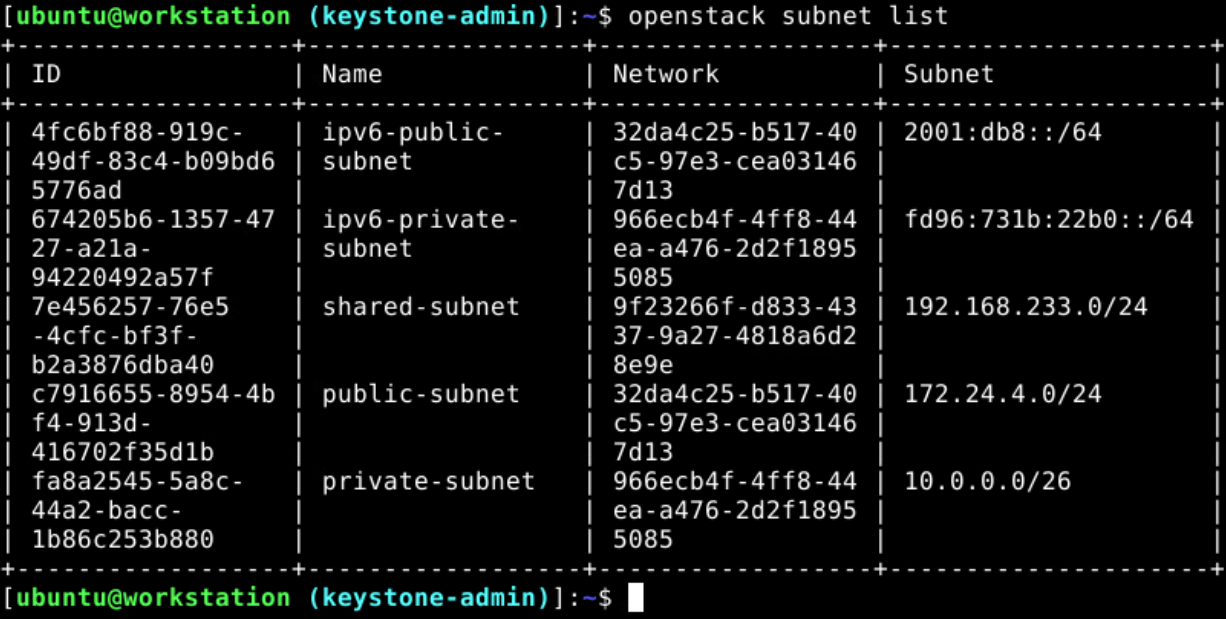
\includegraphics[width=\linewidth]{images/part1/step7.png}
    \end{center}

    \item Use \texttt{nano} to edit the \textbf{\texttildemid/keystonerc-superuser} file. Change the
    \texttt{OS\_USERNAME} to \textbf{superuser}, and change the \texttt{OS\_PROJECT\_NAME} to \textbf{prod}. The file
    should match the the contents shown below. Press \textbf{CTRL+X} to exit the file, then press \textbf{Y} and then
    \textbf{ENTER} to save the changes to the file.
\begin{lstlisting}
ubuntu@workstation:~$ nano ~/keystonerc-superuser
\end{lstlisting}    

    \begin{center}
        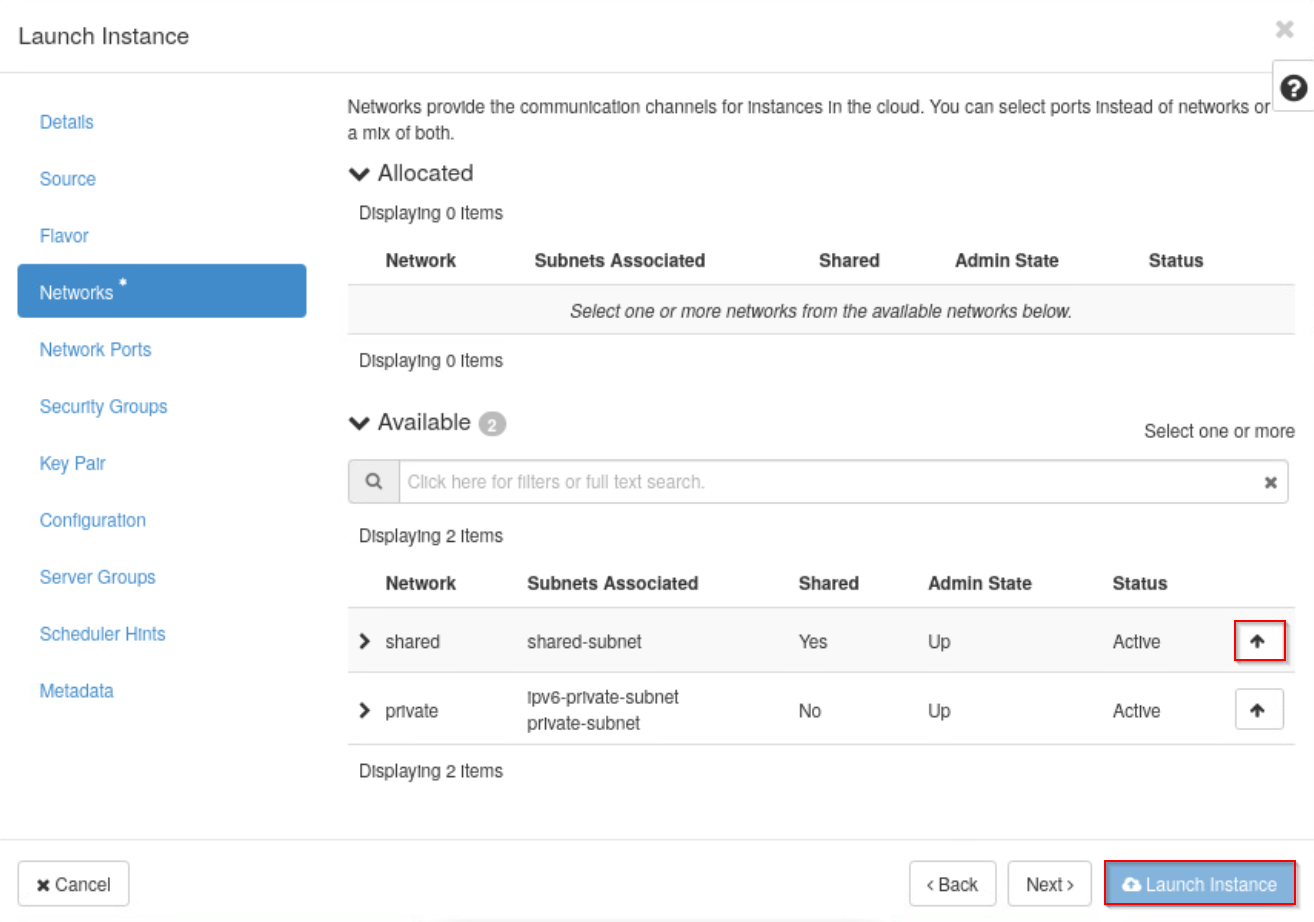
\includegraphics[width=\linewidth]{images/part1/step8.png}
    \end{center}

    \item Now, create a non-privileged user called \textbf{cloud-lab} with the password \textbf{secret}.
\begin{lstlisting}
ubuntu@workstation:~$ openstack user create \
> --project prod \
> --password secret \
> --email ubuntu@workstation.lab.example.com \
> cloud-lab
\end{lstlisting}

    \begin{center}
        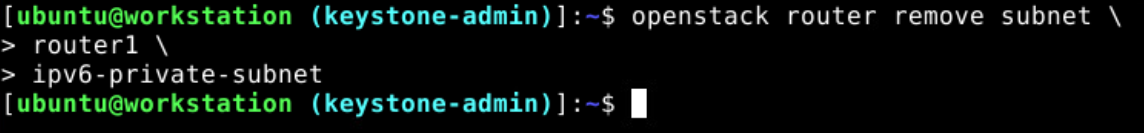
\includegraphics[width=\linewidth]{images/part1/step9.png}
    \end{center}

    \item Assign \textbf{cloud-lab} the \textbf{member} role in the \textbf{prod} project so that it can perform actions
    in that project.
\begin{lstlisting}
ubuntu@workstation:~$ openstack role add \
> --project prod \
> --user cloud-lab \
> member
\end{lstlisting}

    \begin{center}
        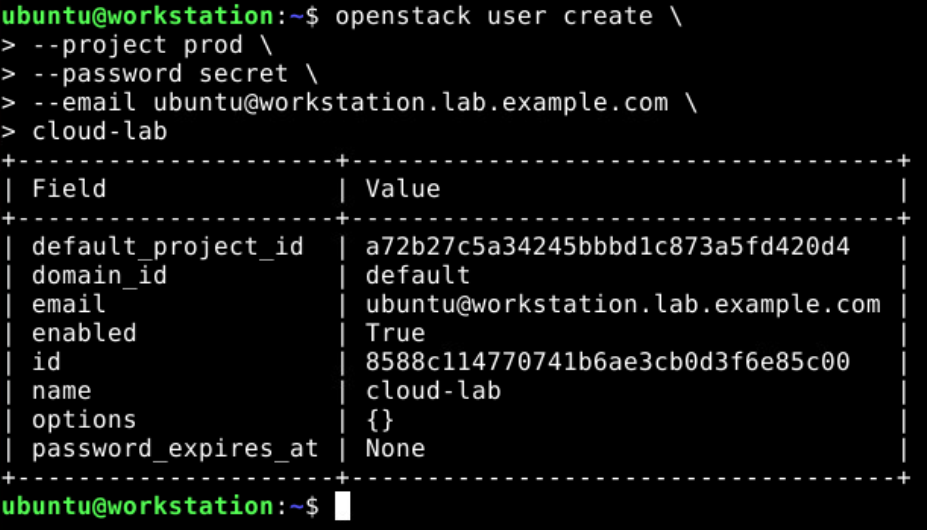
\includegraphics[width=\linewidth]{images/part1/step10.png}
    \end{center}

    \item Copy the keystone credentials file \textbf{\texttildemid/keystonerc-superuser} to
    \textbf{\texttildemid/keystonerc-cloud-lab}.
\begin{lstlisting}
ubuntu@workstation:~$ cp ~/keystonerc-superuser ~/keystonerc-cloud-lab
\end{lstlisting}

    \begin{center}
        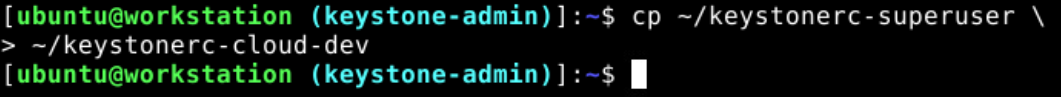
\includegraphics[width=\linewidth]{images/part1/step11.png}
    \end{center}

    \item Use \texttt{nano} to edit the \textbf{\texttildemid/keystonerc-cloud-lab} file. Change the
    \texttt{OS\_USERNAME} to \textbf{cloud-lab}. The file should match the contents shown below. Press \textbf{CTRL+X}
    to exit the file, then press \textbf{Y} and then \textbf{ENTER} to save the changes to the file.
\begin{lstlisting}
ubuntu@workstation:~$ nano ~/keystonerc-cloud-lab
\end{lstlisting}

    \begin{center}
        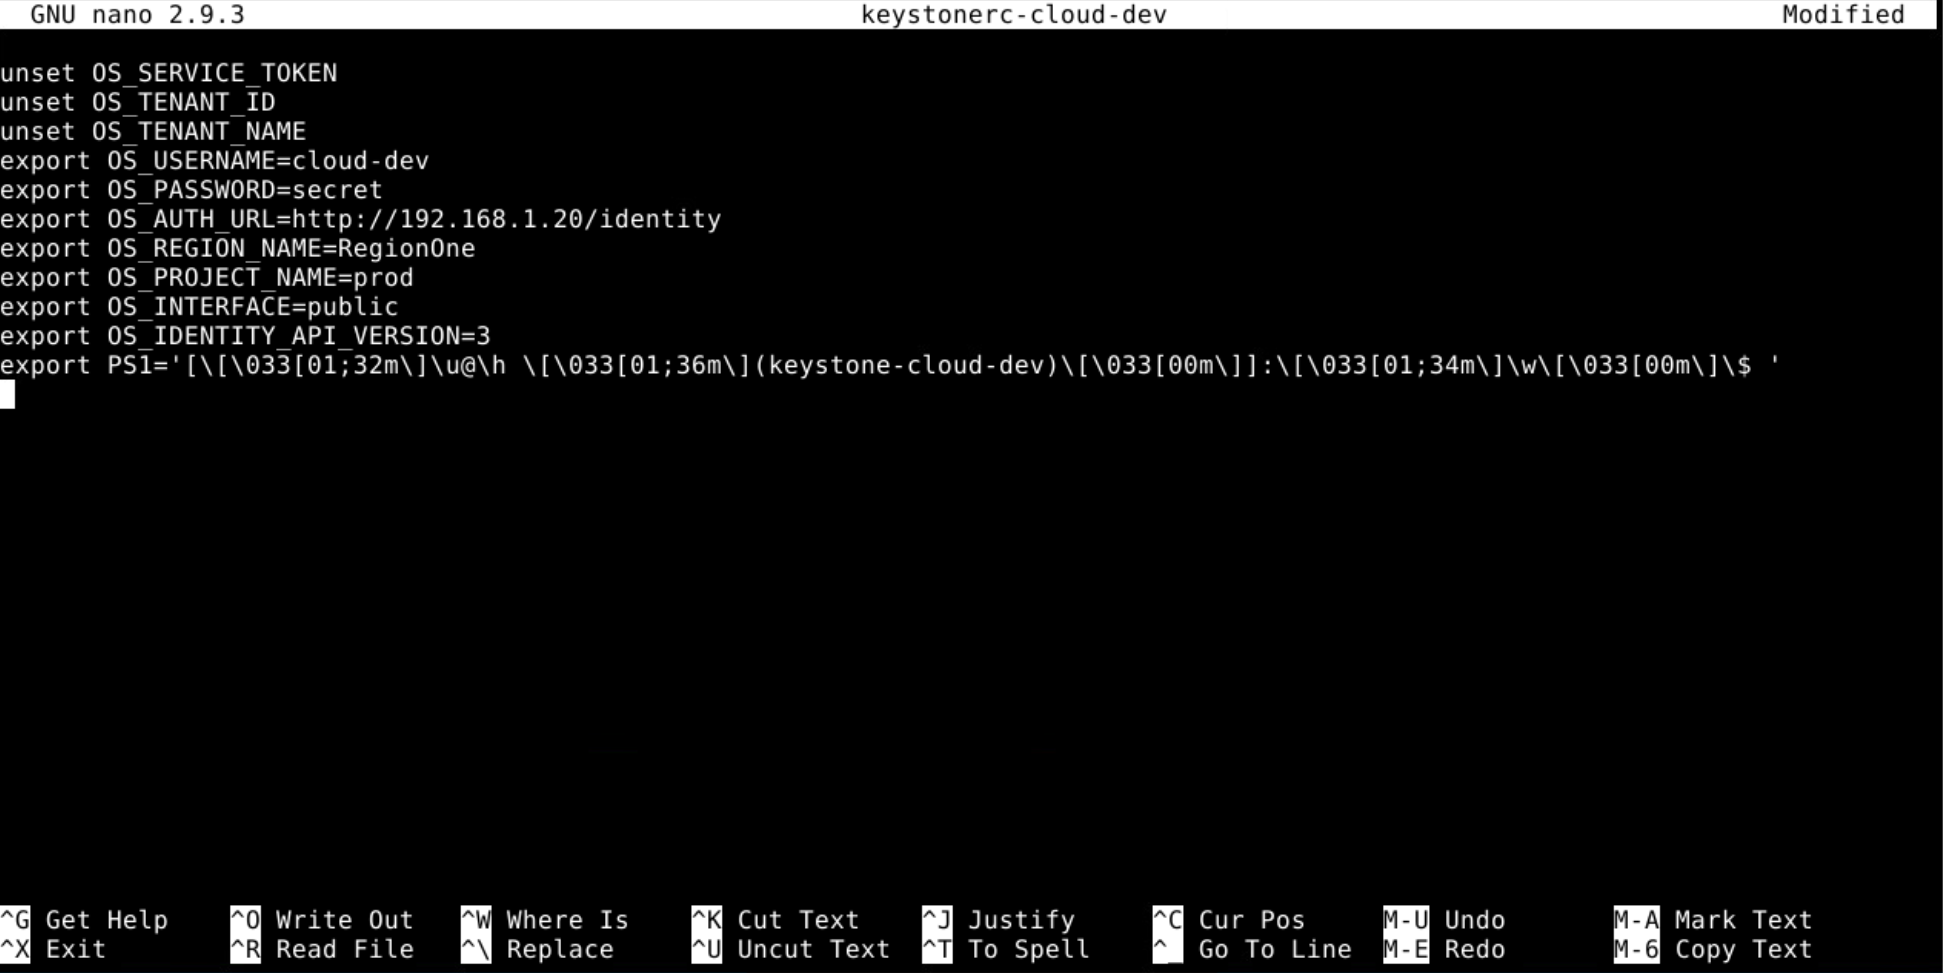
\includegraphics[width=\linewidth]{images/part1/step12.png}
    \end{center}

    \item Now, source the \textbf{keystonerc-superuser} keystone file to begin working with admin privileges in the
    \textbf{prod} project.
\begin{lstlisting}
ubuntu@workstation:~$ source ~/keystonerc-superuser
\end{lstlisting}

    \begin{center}
        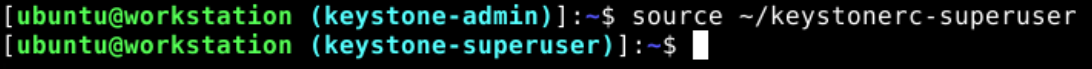
\includegraphics[width=\linewidth]{images/part1/step13.png}
    \end{center}

    \item Before making an external network for the project, the existing one must be deleted. Before the existing
    external network can be deleted, the router needs to be deleted, which requires first deleting its interfaces.
    First, show the details of the router \textbf{router1} to find the interfaces to delete.
\begin{lstlisting}
ubuntu@workstation:~$ openstack router show router1
\end{lstlisting}

    \begin{center}
        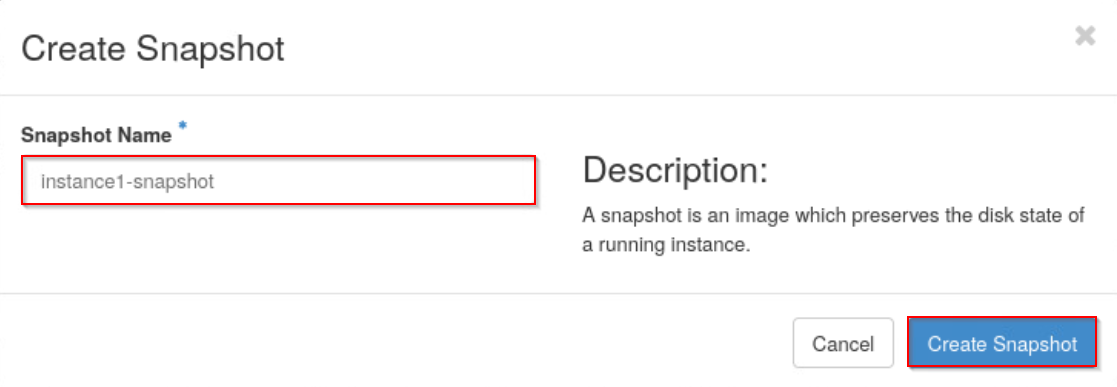
\includegraphics[width=\linewidth]{images/part1/step14.png}
    \end{center}

    \item Next, delete the two interfaces on the router using the \texttt{port\_id} values from the output of the
    previous step.
\begin{lstlisting}
ubuntu@workstation:~$ openstack router remove port \
> router1 \
> 5290b8a9-4f26-415f-b134-459cb139a906
ubuntu@workstation:~$ openstack router remove port \
> router1 \
> 5c97ebfb-d998-413e-998b-f375171b363f
\end{lstlisting}

    \begin{center}
        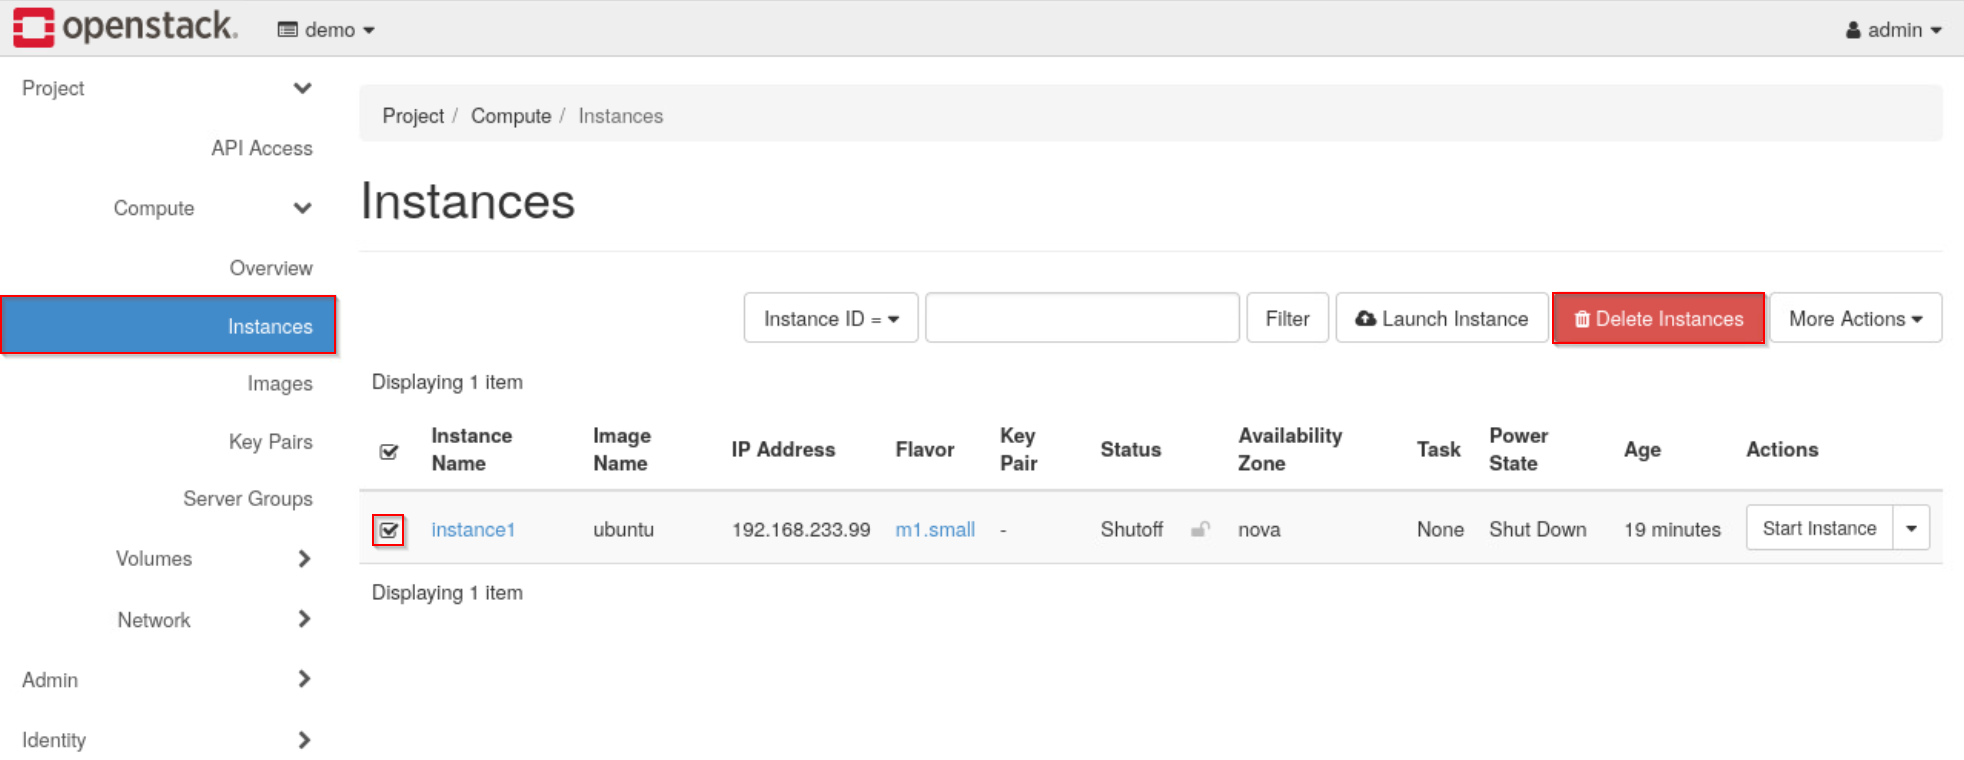
\includegraphics[width=\linewidth]{images/part1/step15.png}
    \end{center}

    \begin{notebox}{}
        The actual IDs may differ from this example.
    \end{notebox}

    \begin{tipbox}{}
        You can copy a string from the terminal by selecting it with the mouse and pressing \textbf{Ctrl+Shift+C}, and
        you can paste to the terminal by pressing \textbf{Ctrl+Shift+V}.
    \end{tipbox}

    \item Now, \textbf{router1} can be deleted.
\begin{lstlisting}
ubuntu@workstation:~$ openstack router delete router1
\end{lstlisting}

    \begin{center}
        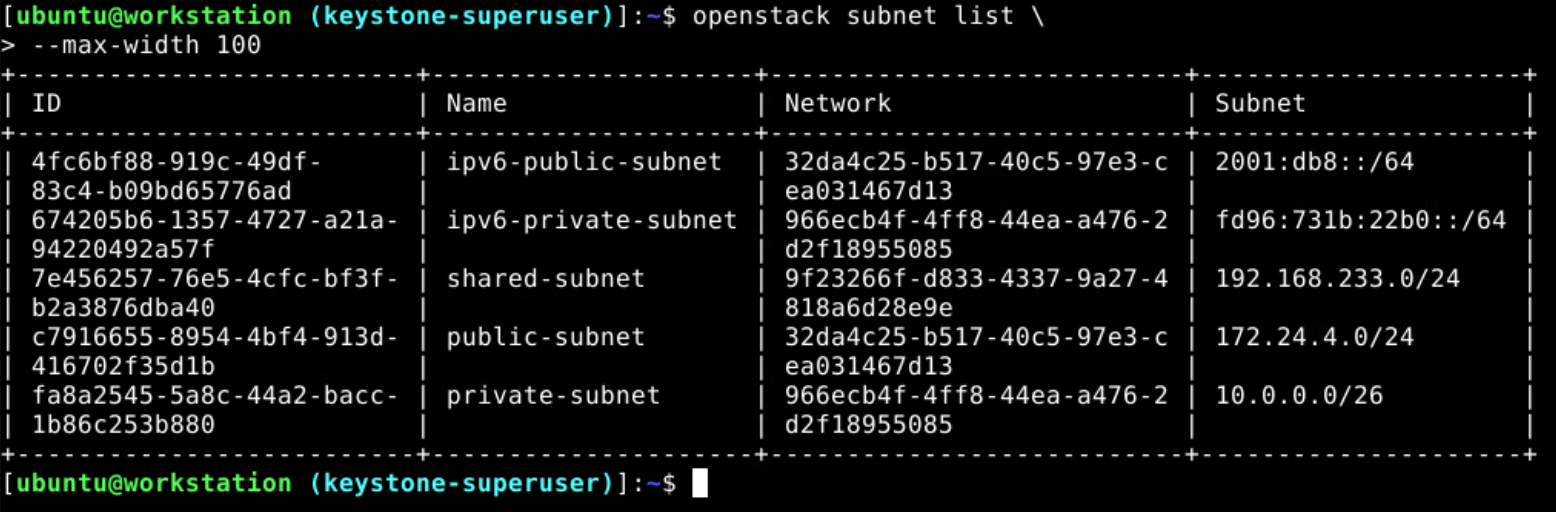
\includegraphics[width=\linewidth]{images/part1/step16.png}
    \end{center}

    \item Finally, delete the existing external network named \textbf{public}.
\begin{lstlisting}
ubuntu@workstation:~$ openstack network delete public
\end{lstlisting}

    \begin{center}
        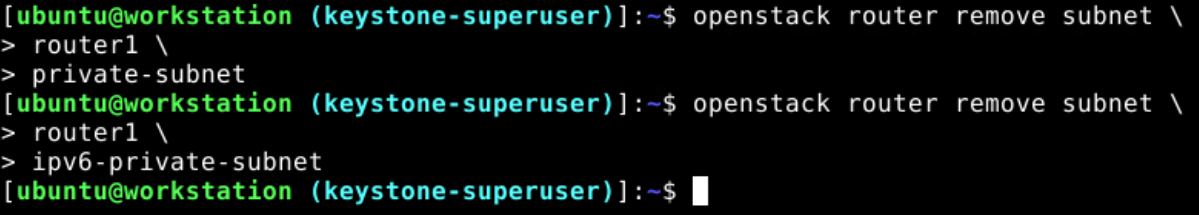
\includegraphics[width=\linewidth]{images/part1/step17.png}
    \end{center}

    \item Create an external, shared network called \textbf{external}.
\begin{lstlisting}
ubuntu@workstation:~$ openstack network create external \
> --external --share \
> --provider-network-type flat \
> --provider-physical-network public
\end{lstlisting}

    \begin{center}
        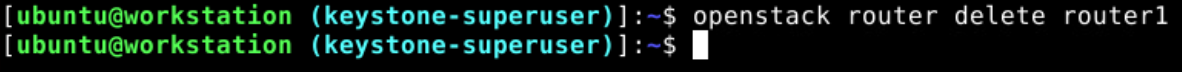
\includegraphics[width=\linewidth]{images/part1/step18.png}
    \end{center}

    \item Create the \textbf{external\_subnet} subnet in the \textbf{172.25.250.0/24} range. Make the floating IP
    allocation pool range from \textbf{172.25.250.25} to \textbf{172.250.250.30}, and allow DHCP. Set both the gateway
    and DNS nameserver addresses to \textbf{172.25.250.254}.
\begin{lstlisting}
ubuntu@workstation:~$ openstack subnet create \
> --subnet-range 172.25.250.0/24 \
> --allocation-pool start=172.25.250.25,end=172.25.250.30 \
> --dhcp --network external \
> --gateway 172.25.250.254 \
> --dns-nameserver 172.25.250.254 external_subnet
\end{lstlisting}

    \begin{center}
        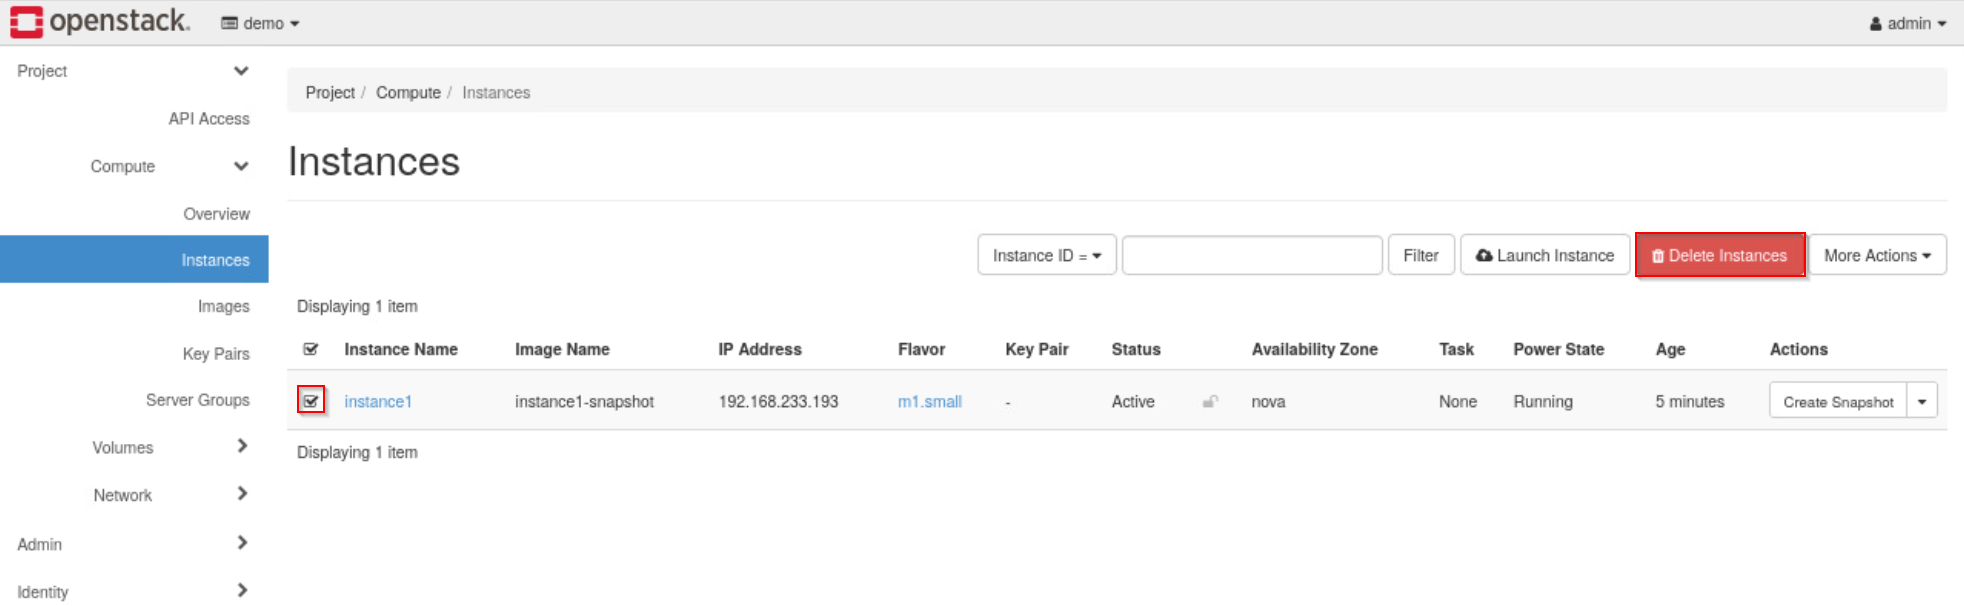
\includegraphics[width=\linewidth]{images/part1/step19.png}
    \end{center}

    \item Source the \textbf{~/keystonerc-cloud-lab} keystone credentials file.
\begin{lstlisting}
ubuntu@workstation:~$ source ~/keystonerc-cloud-lab
\end{lstlisting}

    \begin{center}
        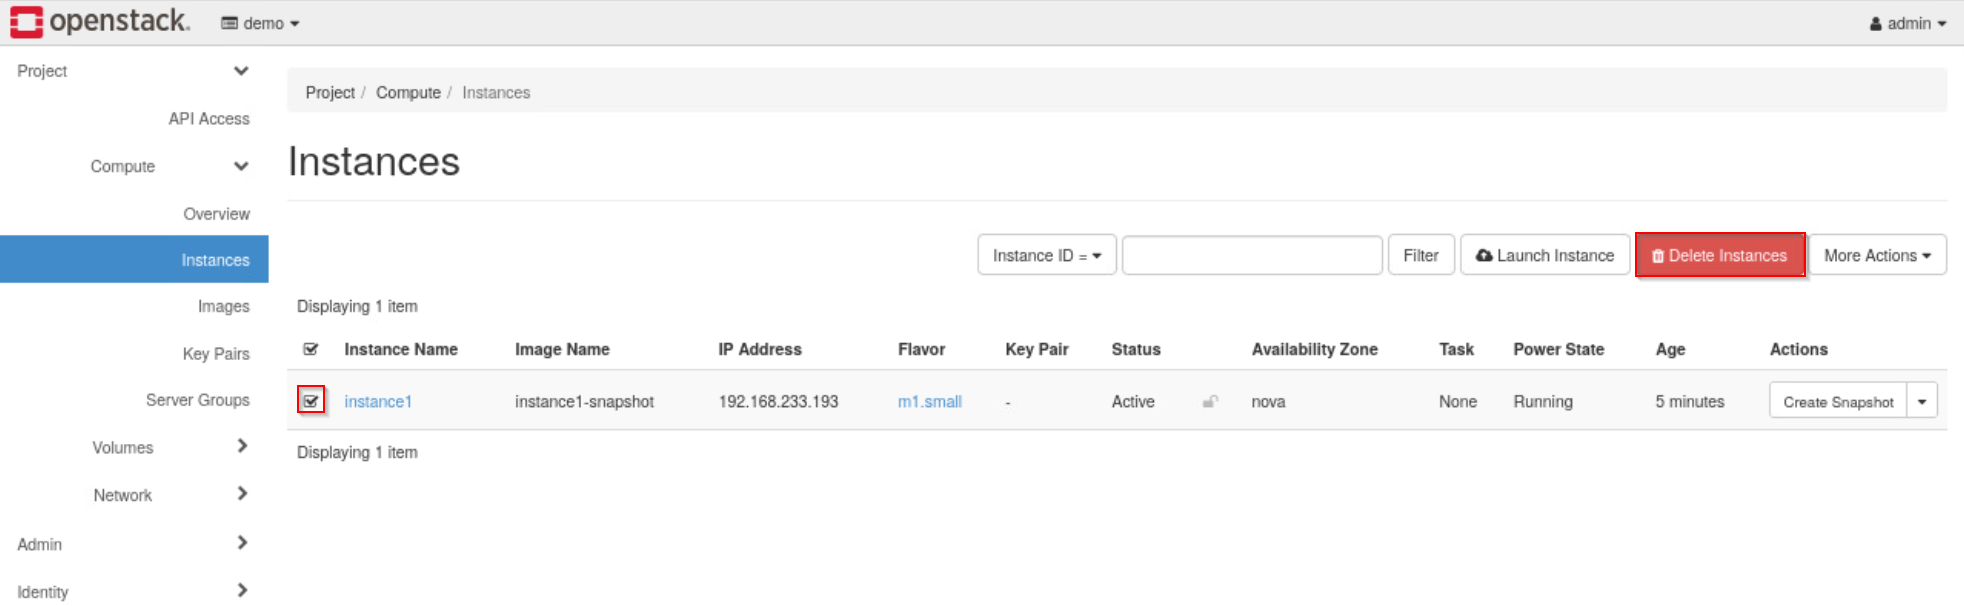
\includegraphics[width=\linewidth]{images/part1/step20.png}
    \end{center}

    \item Create an internal network called \textbf{net1}.
\begin{lstlisting}
ubuntu@workstation:~$ openstack network create net1
\end{lstlisting}

    \begin{center}
        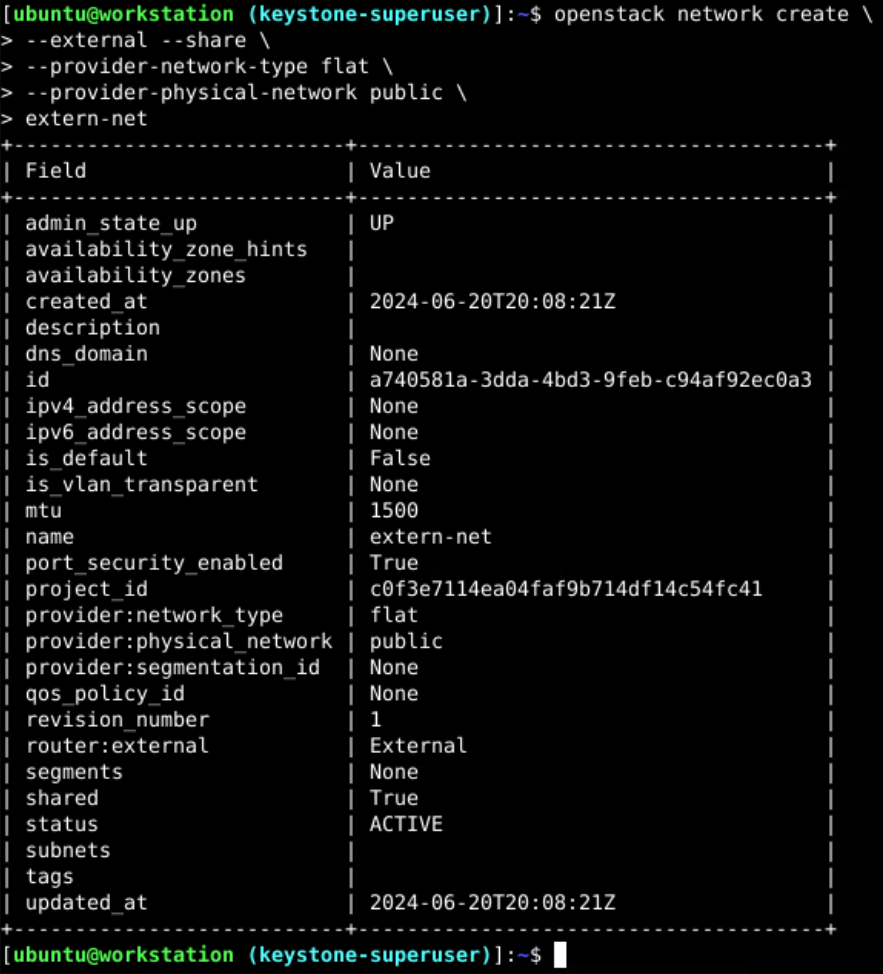
\includegraphics[width=\linewidth]{images/part1/step21.png}
    \end{center}

    \item Create a subnet for \textbf{net1} called \textbf{subnet1} in the \textbf{192.168.0.0/24} range. Allow DHCP on
    the subnet.
\begin{lstlisting}
ubuntu@workstation:~$ openstack subnet create \
> --subnet-range 192.168.0.0/24 \
> --network net1 subnet1
\end{lstlisting}

    \begin{center}
        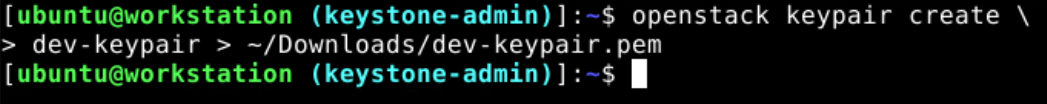
\includegraphics[width=\linewidth]{images/part1/step22.png}
    \end{center}

    \item Create a router named \textbf{router1} so that the internal and external networks can be connected.
\begin{lstlisting}
ubuntu@workstation:~$ openstack router create router1
\end{lstlisting}

    \begin{center}
        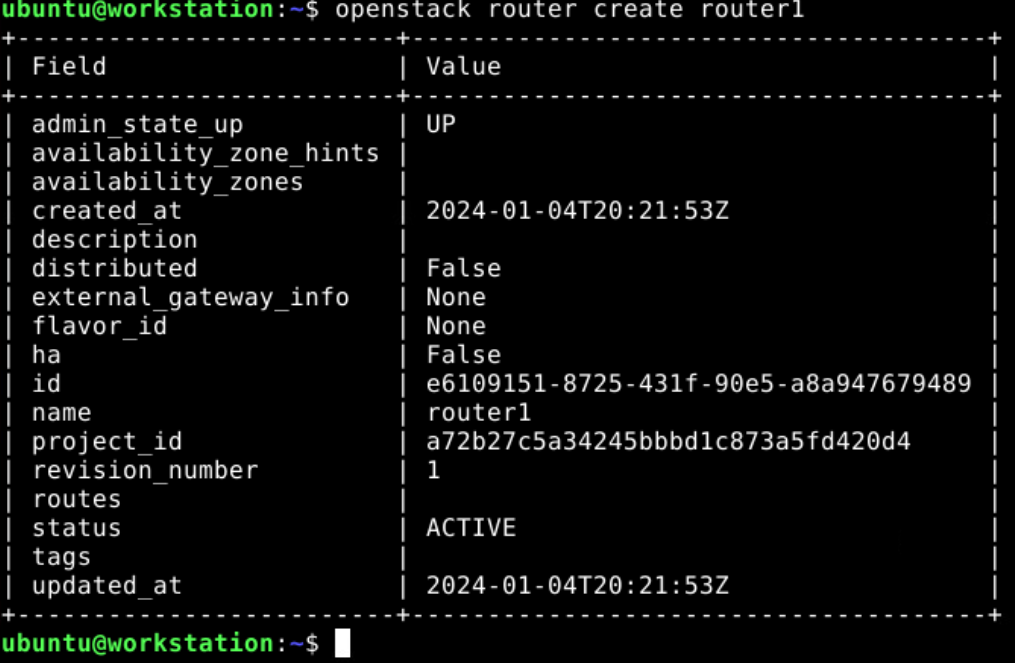
\includegraphics[width=\linewidth]{images/part1/step23.png}
    \end{center}

    \item Add a port to the router for the internal network.
\begin{lstlisting}
ubuntu@workstation:~$ openstack router add subnet router1 subnet1
\end{lstlisting}

    \begin{center}
        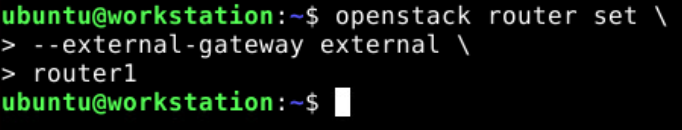
\includegraphics[width=\linewidth]{images/part1/step24.png}
    \end{center}

    \item Set the external network as the gateway for the router.
\begin{lstlisting}
ubuntu@workstation:~$ openstack router set \
> --external-gateway external \
> router1
\end{lstlisting}

    \begin{center}
        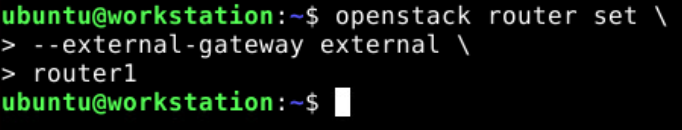
\includegraphics[width=\linewidth]{images/part1/step25.png}
    \end{center}

    \item Allocate a floating IP address from the \textbf{external} network for hte \textbf{prod} project.
\begin{lstlisting}
ubuntu@workstation:~$ openstack floating ip create external
\end{lstlisting}

    \begin{center}
        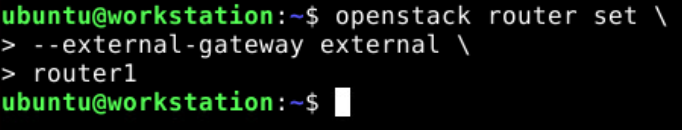
\includegraphics[width=\linewidth]{images/part1/step26.png}
    \end{center}

    \item Generate a key pair for the \textbf{cloud-lab} user named \textbf{key1}.
\begin{lstlisting}
ubuntu@workstation:~$ openstack keypair create \
> key1 > ~/Downloads/key1.pem
\end{lstlisting}

    \begin{center}
        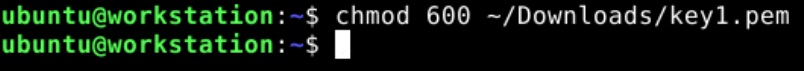
\includegraphics[width=\linewidth]{images/part1/step27.png}
    \end{center}

    \item Change the permissions of the key pair file so that only the \textbf{ubuntu} user has read and write
    permissions.
\begin{lstlisting}
ubuntu@workstation:~$ chmod 600 ~/Downloads/key1.pem
\end{lstlisting}

    \begin{center}
        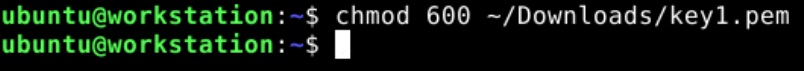
\includegraphics[width=\linewidth]{images/part1/step28.png}
    \end{center}

    \item Create a security group named \textbf{sg1} for the \textbf{prod} project.
\begin{lstlisting}
ubuntu@workstation:~$ openstack security group create \
> --description "SSH, ICMP, and FTP" sg1
\end{lstlisting}    

    \begin{center}
        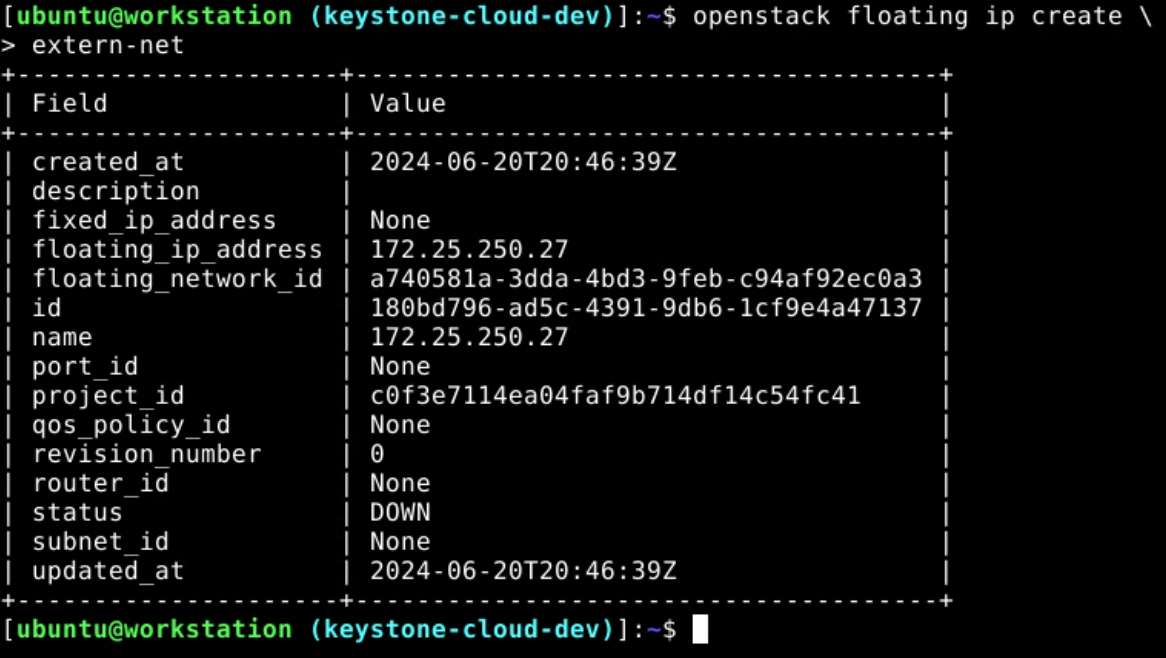
\includegraphics[width=\linewidth]{images/part1/step29.png}
    \end{center}

    \item Create a security group rule to allow \textbf{SSH} traffic from any IP address. SSH uses the TCP protocol on
    port 22 by default.
\begin{lstlisting}
ubuntu@workstation:~$ openstack security group \
> rule create \
> --proto tcp --remote-ip 0.0.0.0/0 --dst-port 22:22 sg1
\end{lstlisting}

    \begin{center}
        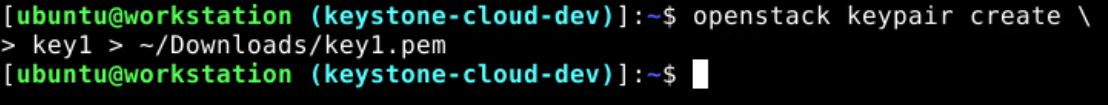
\includegraphics[width=\linewidth]{images/part1/step30.png}
    \end{center}

    \item Create a security group rule to allow \textbf{ICMP} traffic from any IP address.
\begin{lstlisting}
ubuntu@workstation:~$ openstack security group \
> rule create \
> --proto icmp --remote-ip 0.0.0.0/0 sg1
\end{lstlisting}

    \begin{center}
        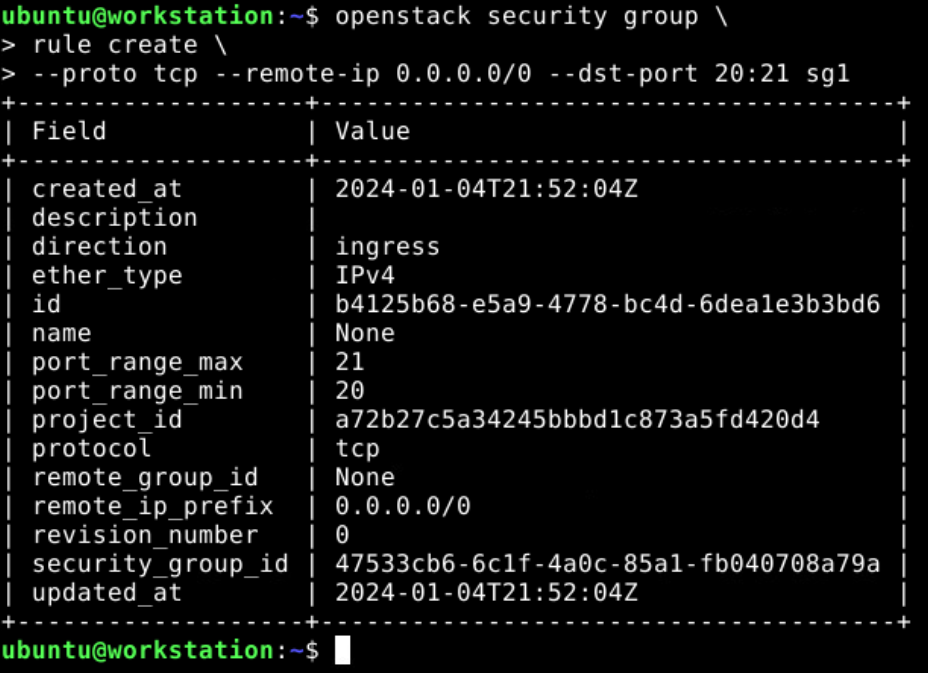
\includegraphics[width=\linewidth]{images/part1/step31.png}
    \end{center}

    \item Create a security group rule to allow \textbf{FTP} traffic from any IP address. FTP uses the TCP protocol on
    port 20 (data channel) and port 21 (control channel).
\begin{lstlisting}
ubuntu@workstation:~$ openstack security group \
> rule create \
> --proto tcp --remote-ip 0.0.0.0/0 --dst-port 20:21 sg1
\end{lstlisting}

    \begin{center}
        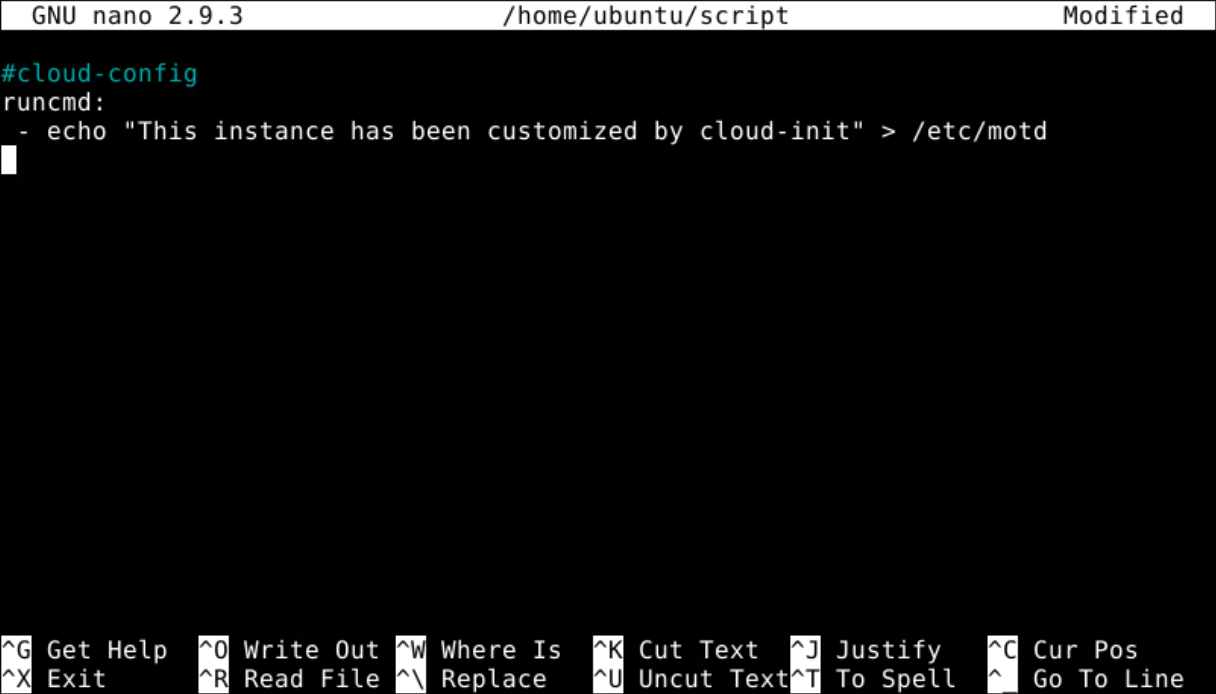
\includegraphics[width=\linewidth]{images/part1/step32.png}
    \end{center}

    \item Create an image named \textbf{ftp} with the file \textbf{~/Downloads/ftp.img}.
\begin{lstlisting}
ubuntu@workstation:~$ openstack image create \
> --disk-format qcow2 \
> --file ~/Downloads/ftp.img \
> ftp
\end{lstlisting}

\begin{center}
    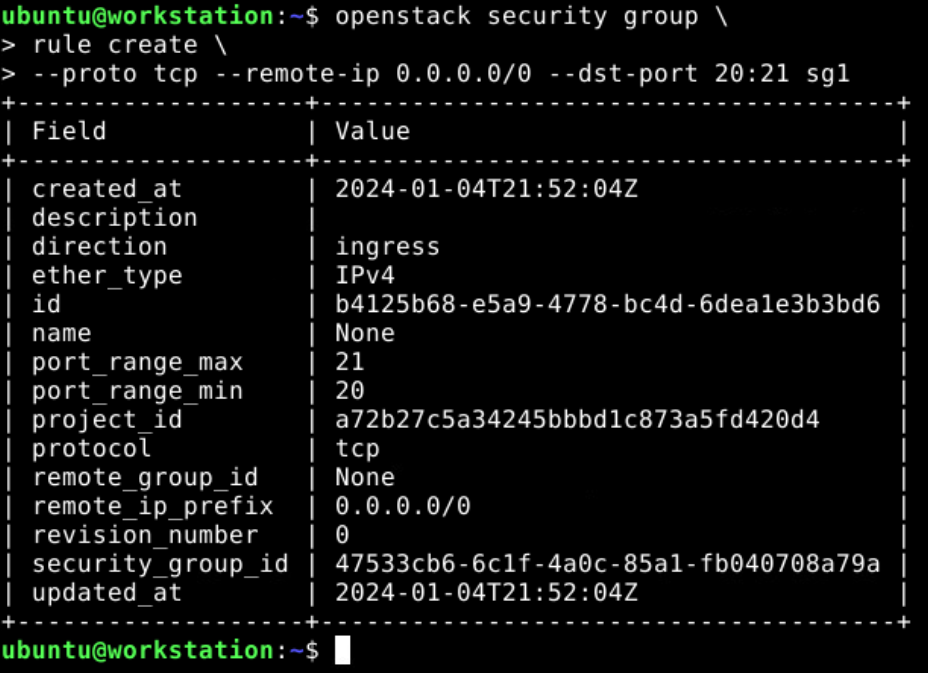
\includegraphics[width=\linewidth]{images/part1/step33.png}
\end{center}

    \item The FTP server instance is almost ready to be launched. First, use \texttt{nano} to create a file named
    \texttt{script} in the home directory. Be sure it has the correct indentation and matches the contents shown below.
    Press \textbf{CTRL+X} to exit the file, then press \textbf{Y} and then \textbf{ENTER} to save the changes to the
    file.
\begin{lstlisting}
ubuntu@workstation:~$ nano ~/script
\end{lstlisting}
\begin{lstlisting}
#cloud-config
runcmd:
 - echo "This instance has been customized by cloud-init" > /etc/motd
\end{lstlisting}

    \begin{center}
        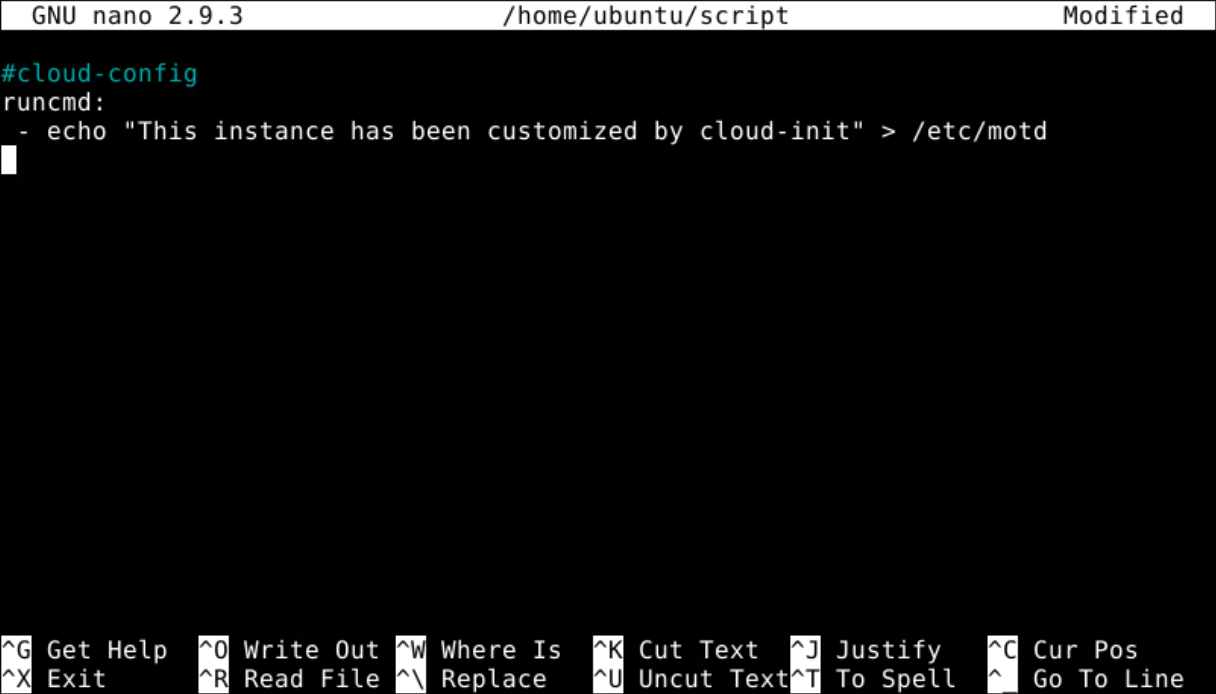
\includegraphics[width=\linewidth]{images/part1/step34.png}
    \end{center}

    \begin{notebox}{}
        This \texttt{cloud-init} script writes to the ``message of the day'' file, and its contents will be displayed
        upon a successful login.
    \end{notebox}

    \item Create an instance named \textbf{ftp\_server} using \textbf{net1} for the internal network, \textbf{m1.small}
    as the flavor, and \textbf{ubuntu} as the image.
\begin{lstlisting}
ubuntu@workstation:~$ openstack server create \
> --image ftp \
> --flavor m1.small \
> --security-group sg1 \
> --user-data ~/script \
> --key-name key1 \
> --nic net-id=net1 \
> --wait ftp_server
\end{lstlisting}

    \begin{center}
        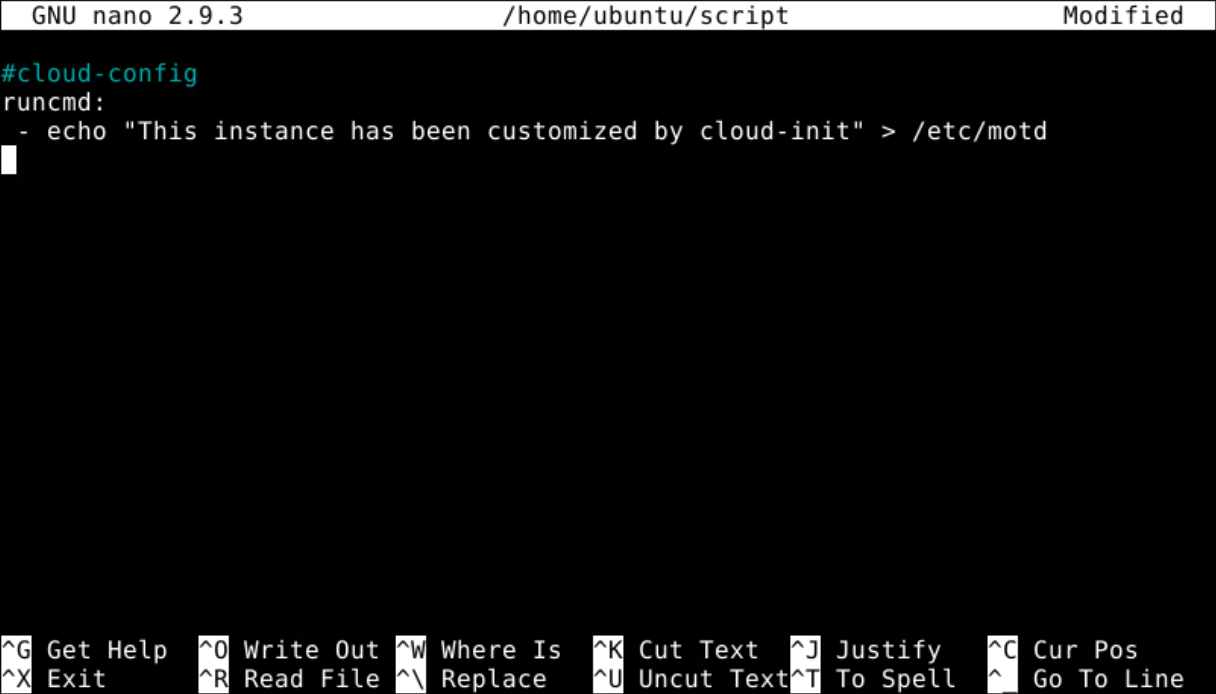
\includegraphics[width=\linewidth]{images/part1/step35.png}
    \end{center}

    \item Ensure that the instance state is \textbf{ACTIVE}.
\begin{lstlisting}
ubuntu@workstation:~$ openstack server list
\end{lstlisting}

    \begin{center}
        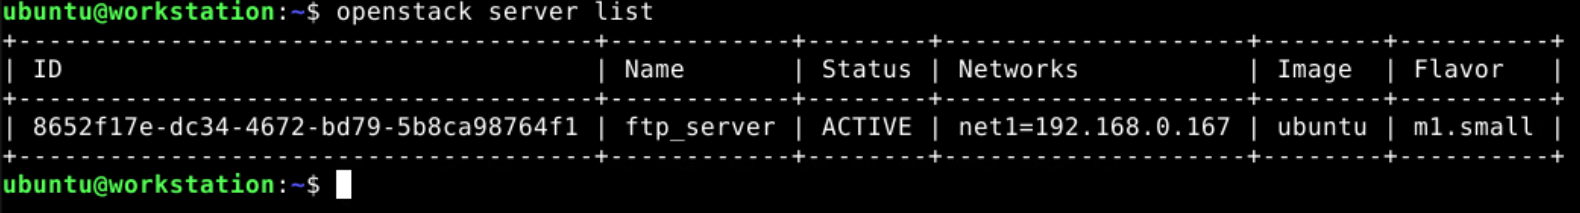
\includegraphics[width=\linewidth]{images/part1/step36.png}
    \end{center}

    \item When the instance state is \textbf{ACTIVE}, list the floating IP addresses available.
\begin{lstlisting}
ubuntu@workstation:~$ openstack floating ip list
\end{lstlisting}

    \begin{center}
        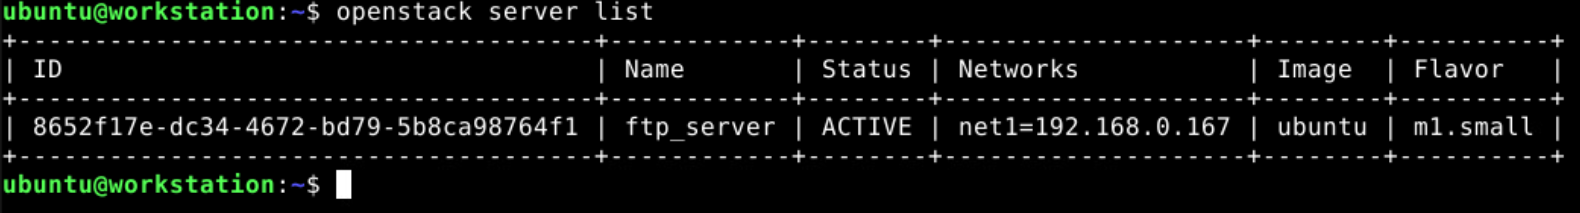
\includegraphics[width=\linewidth]{images/part1/step37.png}
    \end{center}

    \item Associate an open floating IP address to the instance.
\begin{lstlisting}
ubuntu@workstation:~$ openstack server add \
> floating ip ftp_server 172.25.250.30
\end{lstlisting}

    \begin{center}
        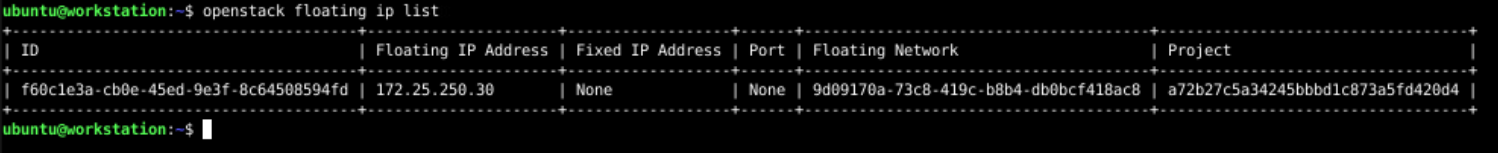
\includegraphics[width=\linewidth]{images/part1/step38.png}
    \end{center}

    \begin{notebox}{}
        When associating the floating IP, make sure to use the IP address that appears for you in the previous step as
        it may differ from this example.
    \end{notebox}

    \item Use the \textbf{\texttt{scp}} command to copy the \textbf{\texttildemid/Downloads/key1.pem} file to the
    \textbf{devstack} machine. When prompted to enter the password for \textbf{ubuntu@192.168.1.20}, enter
    \textbf{ubuntu}.
\begin{lstlisting}
ubuntu@workstation:~$ scp ~/Downloads/key1.pem \
> ubuntu@192.168.1.20:~/key1.pem
\end{lstlisting}

    \begin{center}
        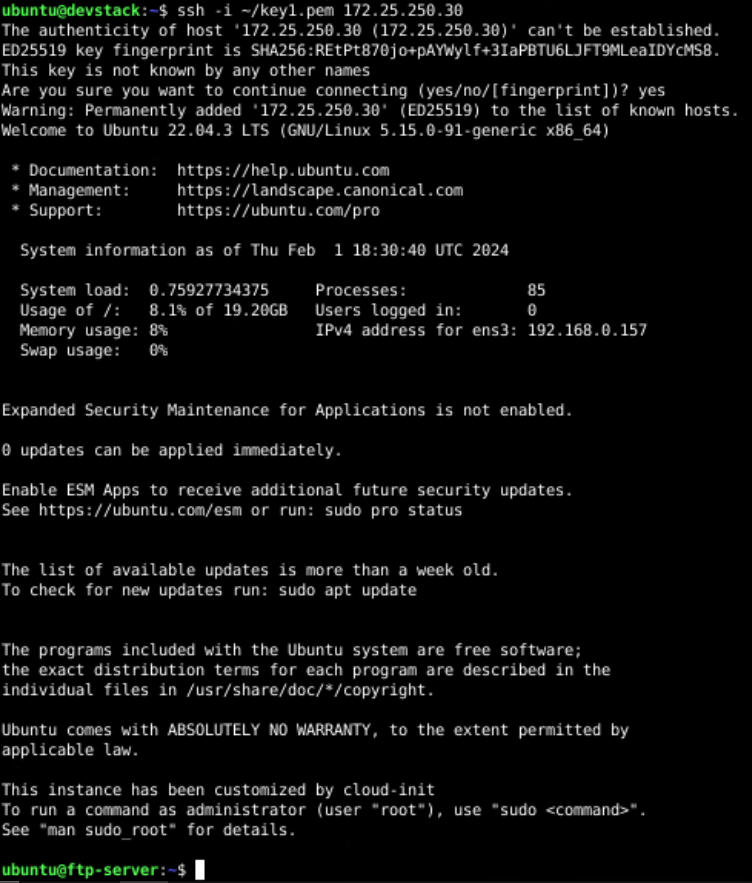
\includegraphics[width=\linewidth]{images/part1/step39.png}
    \end{center}

    \item SSH into the \textbf{devstack} machine. The password is the same as the last step.
\begin{lstlisting}
ubuntu@workstation:~$ ssh 192.168.1.20
\end{lstlisting}

    \begin{center}
        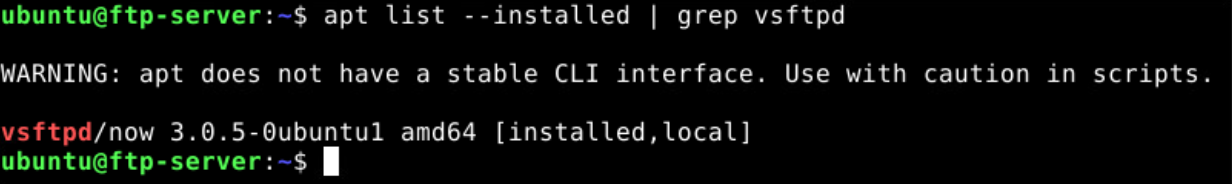
\includegraphics[width=\linewidth]{images/part1/step40.png}
    \end{center}

    \item SSH into the \textbf{ftp\_server} instance using the \textbf{key1} private key. Notice that the message of the
    of the day uploaded with the \texttt{cloud-init} script appears near the bottom of the output.
\begin{lstlisting}
ubuntu@devstack:~$ ssh -i ~/key1.pem 172.25.250.30
\end{lstlisting}

    \begin{center}
        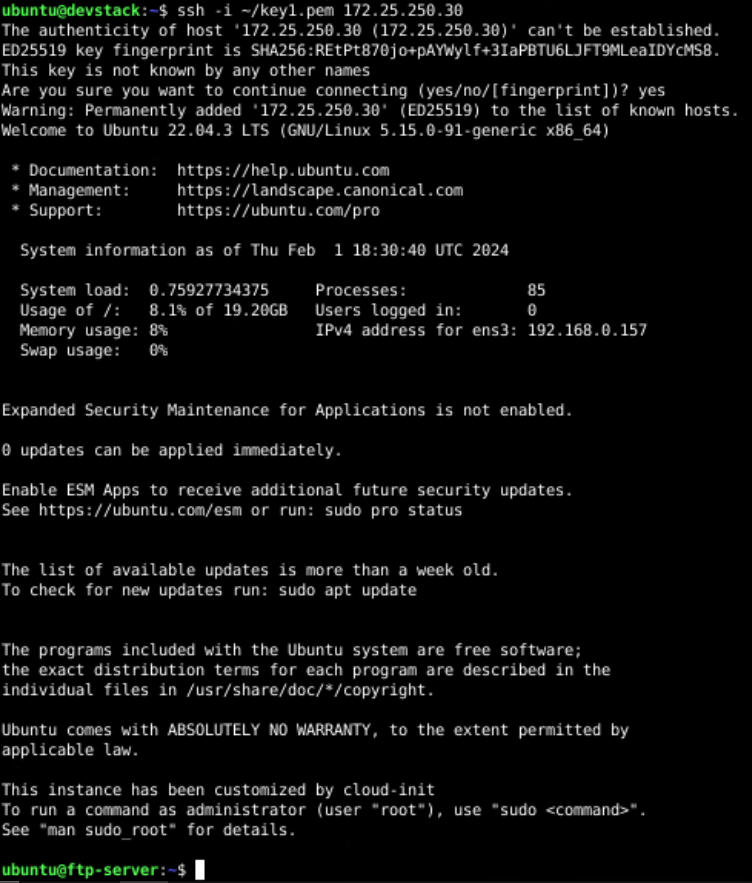
\includegraphics[width=\linewidth]{images/part1/step41.png}
    \end{center}

    \begin{notebox}{}
        The IP address may differ slightly from this example. Make sure to use the floating IP address that you created.
    \end{notebox}

    \begin{notebox}{}
        It may take several minutes for the instance to fully boot and be available for an SSH connection.
    \end{notebox}

    \item Verify that the \texttt{vsftpd} package is installed.
\begin{lstlisting}
ubuntu@ftp-server:~$ apt list --installed | grep vsftpd
\end{lstlisting}

    \begin{center}
        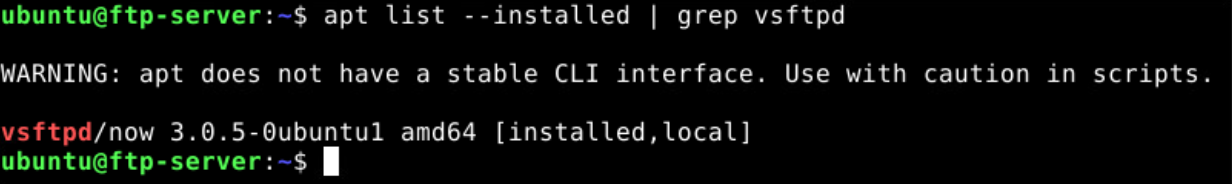
\includegraphics[width=\linewidth]{images/part1/step42.png}
    \end{center}

    \item Use \texttt{nano} to edit the \textbf{/etc/vsftpd.conf} configuration file and uncomment the following
    variables by deleting the ``\texttt{\#}'' character that comes before them: \texttt{anonymous\_enable},
    \texttt{write\_enable}, \texttt{anon\_upload\_enable}, and \texttt{anon\_mkdir\_write\_enable}. Then, append the
    following lines: \texttt{allow\_writeable\_chroot=YES} and \texttt{anon\_root=/var/ftp}. The content of the file
    should resemble the output given below.
\begin{lstlisting}
ubuntu@ftp-server:~$ sudo nano /etc/vsftpd.conf
\end{lstlisting}
\begin{lstlisting}
anonymous_enable=YES
write_enable=YES
anon_upload_enable=YES
anon_mkdir_write_enable=YES
allow_writeable_chroot=YES
anon_root=/var/ftp
\end{lstlisting}

    \begin{center}
        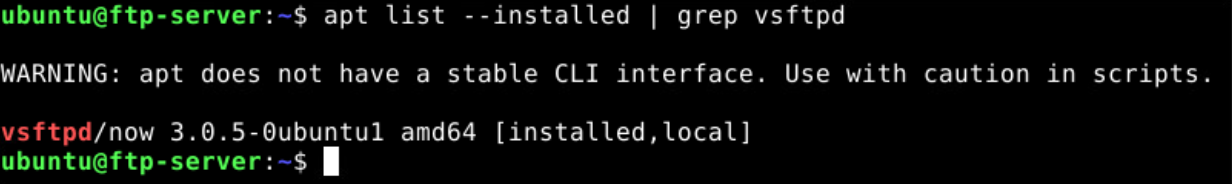
\includegraphics[width=\linewidth]{images/part1/step43.png}
    \end{center}

    \item Create a folder for anonymous FTP users.
\begin{lstlisting}
ubuntu@ftp-server:~$ sudo mkdir -p /var/ftp/pub
\end{lstlisting}

    \begin{center}
        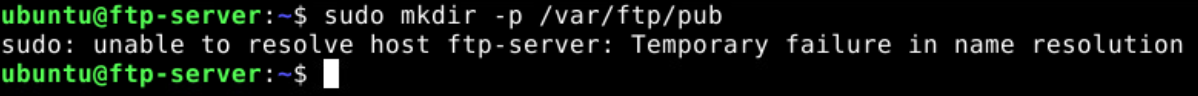
\includegraphics[width=\linewidth]{images/part1/step44.png}
    \end{center}

    \item Remove all ownership from the root FTP folder and remove write permissions from this folder.
\begin{lstlisting}
ubuntu@ftp-server:~$ sudo chown nobody:nogroup /var/ftp
ubuntu@ftp-server:~$ sudo chmod a-w /var/ftp
\end{lstlisting}

    \begin{center}
        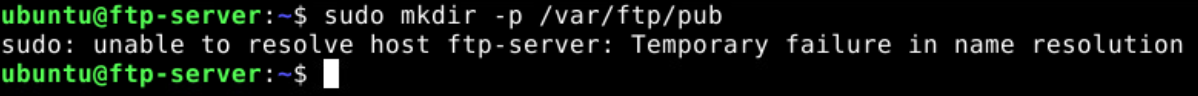
\includegraphics[width=\linewidth]{images/part1/step45.png}
    \end{center}

    \item Change the ownership of the \textbf{/var/ftp/pub} directory so that the \textbf{ftp} user and group owns
    everything within this directory.
\begin{lstlisting}
ubuntu@ftp-server:~$ sudo chown -R ftp. /var/ftp/pub
\end{lstlisting}

    \begin{center}
        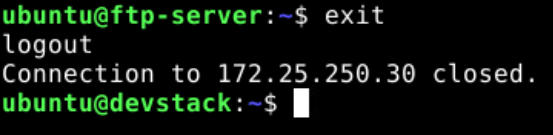
\includegraphics[width=\linewidth]{images/part1/step46.png}
    \end{center}

    \item Restart the \texttt{vsftpd} service so the changes will take effect.
\begin{lstlisting}
ubuntu@ftp-server:~$ sudo systemctl restart vsftpd
\end{lstlisting}

    \begin{center}
        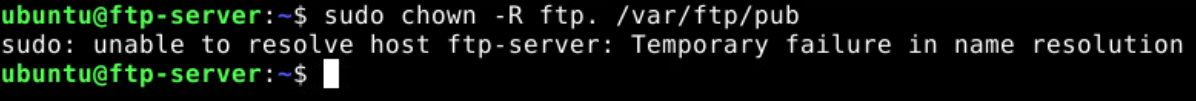
\includegraphics[width=\linewidth]{images/part1/step47.png}
    \end{center}

    \item Exit from the \textbf{ftp\_server} instance.
\begin{lstlisting}
ubuntu@ftp-server:~$ exit
\end{lstlisting}

    \begin{center}
        \includegraphics[width=\linewidth]{images/part1/step48.png}
    \end{center}

    \item From \textbf{workstation}, create a text file named \textbf{test\_file.txt} containing the string ``This is my
    file''.
\begin{lstlisting}
ubuntu@devstack:~$ echo "This is my file" > test_file.txt
\end{lstlisting}

    \begin{center}
        \includegraphics[width=\linewidth]{images/part1/step49.png}
    \end{center}

    \item Open an FTP session to the FTP server and upload the \textbf{test\_file.txt} file. Log out when done. Use
    \textbf{anonymous} as the user and when prompted for the password, press the \textbf{Enter} key for no password
    input. Follow the instructions from the example and summary below.
\begin{lstlisting}
ubuntu@devstack:~$ ftp 172.25.250.30
ftp> passive
ftp> dir
ftp> cd pub
ftp> put test_file.txt test_file.txt
ftp> bye
\end{lstlisting}

    \begin{center}
        \includegraphics[width=\linewidth]{images/part1/step50.png}
    \end{center}

    \begin{notebox}{}
        The IP address may differ slightly from this example. Make sure to use the floating IP address that you created.
    \end{notebox}

    \item SSH into the \textbf{ftp\_server} instance.
\begin{lstlisting}
ubuntu@devstack:~$ ssh -i ~/Downloads/key1.pem cloud-user@172.25.250.30
\end{lstlisting}

    \begin{center}
        \includegraphics[width=\linewidth]{images/part1/step51.png}
    \end{center}

    \item Verify the file uploaded successfully.
\begin{lstlisting}
ubuntu@ftp-server:~$ sudo cat /var/ftp/pub/test_file.txt
\end{lstlisting}

    \begin{center}
        \includegraphics[width=\linewidth]{images/part1/step52.png}
    \end{center}

    \item Exit from the \textbf{ftp\_server} instance.
\begin{lstlisting}
ubuntu@ftp-server:~$ exit
\end{lstlisting}

    \begin{center}
        \includegraphics[width=\linewidth]{images/part1/step53.png}
    \end{center}

    \item The lab is now complete.

\end{enumerate}
\end{document}